\documentclass[11pt,a4paper,oneside]{book}
\usepackage[top=2.8cm,bottom=2.8cm,left=3cm,right=2.6cm]{geometry}
\usepackage[T1]{fontenc}
\usepackage{lmodern}
\usepackage{microtype}
\usepackage{amsmath,amssymb,bm}
\usepackage{graphicx}
\usepackage{booktabs,array,tabularx,longtable}
\usepackage{enumitem}
\usepackage[table]{xcolor}
\usepackage{tikz}
\usepackage{pgfplots}
\pgfplotsset{compat=1.17}
\usepgfplotslibrary{groupplots}
\usetikzlibrary{arrows.meta,positioning,calc,fit}
\usepackage{listings}
\usepackage[most]{tcolorbox}
\usepackage{fancyhdr}
\usepackage{float}
\usepackage{caption}
\usepackage{xurl}
\usepackage[colorlinks=true,linkcolor=blue!50!black,urlcolor=blue!50!black,citecolor=blue!50!black]{hyperref}

% ---------------------------------------------------------------------------
% Istilah Bahasa Indonesia
% ---------------------------------------------------------------------------
\renewcommand{\contentsname}{Daftar Isi}
\renewcommand{\chaptername}{Bab}
\renewcommand{\figurename}{Gambar}
\renewcommand{\tablename}{Tabel}
\renewcommand{\bibname}{Daftar Pustaka}
\renewcommand{\appendixname}{Lampiran}
\renewcommand{\lstlistingname}{Kode}

% ---------------------------------------------------------------------------
% Warna dan kotak
% ---------------------------------------------------------------------------
\definecolor{skdblue}{HTML}{1F3A68}
\definecolor{skdlight}{HTML}{E8EEF7}
\definecolor{skdorange}{HTML}{D9822B}
\definecolor{skdgreen}{HTML}{2E8B57}
\definecolor{skdred}{HTML}{B03A2E}
\definecolor{skdgray}{HTML}{6B7280}

\newcommand{\en}[1]{{\color{skdgray}\textit{#1}}}
\newcommand{\term}[2]{\textbf{#1} \en{(#2)}}
\newcommand{\enchap}[1]{\vspace*{-1.2em}{\Large\en{#1}}\par\vspace{1.5em}}

\newtcolorbox{tujuan}{colback=skdlight,colframe=skdblue,fonttitle=\bfseries,title={Tujuan Pembelajaran \en{\color{white!85!skdblue}/ Learning Objectives}},boxrule=0.6pt,arc=2pt}
\newtcolorbox[auto counter,number within=chapter]{contoh}[1][]{colback=skdgreen!6,colframe=skdgreen,fonttitle=\bfseries,title={Contoh~\thetcbcounter\ifx&#1&\else: #1\fi},boxrule=0.6pt,arc=2pt,breakable}
\newtcolorbox{ringkasan}{colback=skdorange!7,colframe=skdorange,fonttitle=\bfseries,title={Ringkasan \en{\color{white!85!skdorange}/ Summary}},boxrule=0.6pt,arc=2pt,breakable}
\newtcolorbox{catatan}{colback=white,colframe=skdgray,fonttitle=\bfseries,title={Catatan praktik},boxrule=0.5pt,arc=2pt,breakable}

\pgfplotsset{
	skd/.style={axis lines=left,grid=major,grid style={black!10},tick label style={font=\scriptsize},label style={font=\small},legend style={font=\scriptsize,draw=none,fill=white,fill opacity=0.85,text opacity=1},every axis plot/.append style={thick}},
}
\tikzset{
	blk/.style={draw=skdblue,thick,fill=white,rounded corners=2pt,minimum height=0.9cm,minimum width=1.5cm,align=center,font=\small},
	blkd/.style={blk,fill=skdlight},
	sum/.style={draw=skdblue,thick,circle,inner sep=0pt,minimum size=0.45cm},
	sig/.style={-{Stealth[length=2.2mm]},thick,skdblue},
	lbl/.style={font=\scriptsize,text=skdgray},
}

\lstset{basicstyle=\ttfamily\footnotesize,keywordstyle=\color{blue!70!black}\bfseries,commentstyle=\color{green!45!black},frame=single,breaklines=true,columns=fullflexible,keepspaces=true,showstringspaces=false}

\newcommand{\dat}[1]{../slides/data/#1}

% ---------------------------------------------------------------------------
% Header
% ---------------------------------------------------------------------------
\pagestyle{fancy}
\fancyhf{}
\fancyhead[L]{\small\nouppercase{\leftmark}}
\fancyhead[R]{\small TF4015 Sistem Kontrol Diskrit}
\fancyfoot[C]{\thepage}
\setlength{\headheight}{14pt}
\setlist{itemsep=2pt,topsep=4pt}

\begin{document}

\frontmatter
\begin{titlepage}
	\centering
	\vspace*{2cm}
	{\large Program Studi Teknik Fisika\\Fakultas Teknologi Industri\\Institut Teknologi Bandung\par}
	\vspace{3cm}
	{\color{skdblue}\rule{0.85\textwidth}{1.2pt}\par}
	\vspace{0.5cm}
	{\Huge\bfseries Sistem Kontrol Diskrit\par}
	\vspace{0.3cm}
	{\LARGE\en{Discrete-Time Control Systems}\par}
	\vspace{0.4cm}
	{\large Catatan Kuliah TF4015 \,/\, \en{Lecture Notes}\par}
	\vspace{0.5cm}
	{\color{skdblue}\rule{0.85\textwidth}{1.2pt}\par}
	\vfill
	{\large Ir. Estiyanti Ekawati, M.T., Ph.D.\\[2pt] Faqihza Mukhlish, S.T., M.T., Ph.D.\par}
	\vspace{1.5cm}
	{\large Semester I 2026/2027\par}
\end{titlepage}

\chapter*{Prakata}
Catatan kuliah ini menyertai mata kuliah TF4015 Sistem Kontrol Diskrit (3 SKS). Isinya mengikuti Rencana Pembelajaran Semester: satu bab untuk setiap pertemuan tatap muka, dengan Pertemuan 8 dan 16 dipakai untuk ujian. Catatan ini tidak menggantikan buku teks; tujuannya merangkum konsep inti, menunjukkan penurunan yang penting, dan memberi contoh numerik yang konsisten dengan slide kuliah dan modul praktikum.

Sepanjang catatan dipakai satu plant acuan yang sama dengan kit praktikum, yaitu motor DC yang dinormalisasi:
\[
	G_v(s) = \frac{K}{\tau s + 1}\ \text{(kecepatan)},\qquad G_p(s) = \frac{K}{s(\tau s+1)}\ \text{(posisi)},
\]
dengan $K = 1$, $\tau = 0{,}5$\,s, dan waktu cacah $T = 0{,}1$\,s, kecuali disebutkan lain. Dengan demikian setiap metode dapat dibandingkan pada sistem yang sama. Semua angka contoh dan grafik dihitung dengan skrip Python yang disertakan bersama slide (\texttt{scripts/gen\_data.py}).

Bahasa pengantar adalah Bahasa Indonesia. Istilah teknis diberi padanan bahasa Inggris \en{(dalam huruf miring abu-abu)} saat pertama kali muncul, dan setiap bab ditutup dengan ringkasan, daftar istilah kunci, serta latihan.

\paragraph{Buku teks.}
\begin{itemize}
	\item[{[FR]}] Franklin, G.~F., Powell, J.~D., dan Emami-Naeini, A., \textit{Feedback Control of Dynamic Systems}, ed.~8, Pearson, 2018.
	\item[{[OG]}] Ogata, K., \textit{Discrete-Time Control Systems}, ed.~2, Pearson India, 2015.
	\item[{[PH]}] Phillips, C.~L., Nagle, H.~T., dan Chakrabortty, A., \textit{Digital Control System Analysis \& Design}, ed.~4, Pearson, 2014.
\end{itemize}

\tableofcontents

\mainmatter
\chapter{Pendahuluan dan Tinjauan Kontrol Kontinu}
\enchap{Introduction and Review of Continuous-Time Control}

\begin{tujuan}
	Setelah mempelajari bab ini, Anda mampu menjelaskan struktur sistem kontrol digital, meninjau kembali pemodelan dan fungsi transfer sistem kontinu, menghubungkan spesifikasi kinerja dengan lokasi kutub, serta menala pengontrol PID secara heuristik. Bab ini juga menunjukkan mengapa pencacahan menuntut alat analisis baru.
\end{tujuan}

\section{Sistem kontrol digital}
\term{Kontrol}{control} adalah upaya memastikan suatu sistem berperilaku sesuai kriteria perancangannya. Pada sistem kontrol modern, hampir semua pengontrol diwujudkan dalam perangkat lunak yang dijalankan oleh mikrokontroler, PLC, atau komputer. Komputer tidak dapat mengamati sinyal fisik secara terus-menerus; ia hanya membaca sensor pada saat-saat tertentu, menghitung aksi kontrol, lalu menahan aksi itu sampai perhitungan berikutnya.

Struktur umum sistem kontrol digital ditunjukkan pada Gambar~\ref{fig:b1-struktur}. Plant dan aktuator bekerja dalam waktu kontinu dengan sinyal $u(t)$ dan $y(t)$. Komputer bekerja dengan barisan bilangan $u[k]$ dan $y[k]$ yang diperbarui setiap \term{waktu cacah}{sampling period} $T$. Dua antarmuka menghubungkan keduanya: \textit{analog-to-digital converter} (ADC) yang mencacah dan mengkuantisasi pengukuran, serta \textit{digital-to-analog converter} (DAC) yang menahan keluaran digital sebagai tegangan konstan selama satu periode cacah.

\begin{figure}[H]
	\centering
	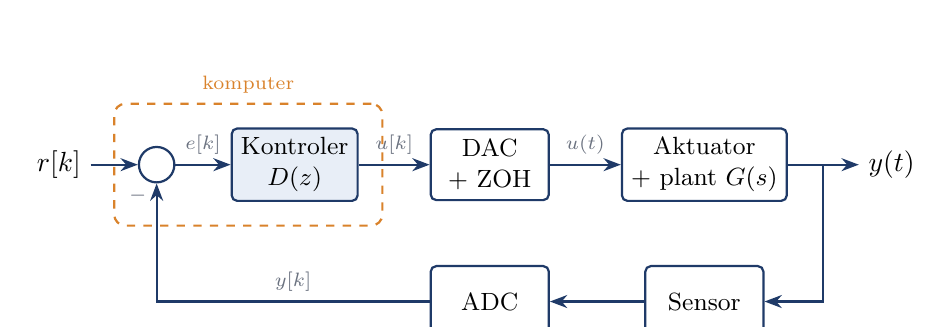
\begin{tikzpicture}[node distance=0.55cm and 0.7cm]
		\node[sum] (s) {};
		\node[left=0.6cm of s] (r) {$r[k]$};
		\node[blkd,right=of s] (c) {Kontroler\\$D(z)$};
		\node[blk,right=0.9cm of c] (dac) {DAC\\+ ZOH};
		\node[blk,right=0.9cm of dac] (p) {Aktuator\\+ plant $G(s)$};
		\node[right=0.9cm of p] (y) {$y(t)$};
		\node[blk,below=0.8cm of p] (sen) {Sensor};
		\node[blk] (adc) at (dac |- sen) {ADC};
		\draw[sig] (r) -- (s);
		\draw[sig] (s) -- node[above,lbl]{$e[k]$} (c);
		\draw[sig] (c) -- node[above,lbl]{$u[k]$} (dac);
		\draw[sig] (dac) -- node[above,lbl]{$u(t)$} (p);
		\draw[sig] (p) -- coordinate[pos=0.5](yt) (y);
		\draw[sig] (yt) |- (sen);
		\draw[sig] (sen) -- (adc);
		\draw[sig] (adc) -| node[pos=0.25,above,lbl]{$y[k]$} node[pos=0.95,left,lbl]{$-$} (s);
		\node[draw=skdorange,dashed,thick,rounded corners,fit=(s)(c),inner sep=0.3cm,label={[font=\scriptsize,text=skdorange]above:komputer}] {};
	\end{tikzpicture}
	\caption{Struktur sistem kontrol digital}
	\label{fig:b1-struktur}
\end{figure}

Pada kit praktikum SKD, kontroler adalah Arduino UNO, DAC adalah MCP4725 yang diikuti penguat dan driver motor, plant adalah motor DC 24\,V, sensornya tachometer dan potensiometer, dan ADC adalah ADC 10-bit internal Arduino. Setiap konsep di kuliah ini akan ditemui kembali secara fisik di kit tersebut.

Kontrol digital menawarkan fleksibilitas (algoritma diubah lewat perangkat lunak), kemampuan menjalankan algoritma kompleks, bebas \textit{drift} komponen, serta kemudahan pencatatan data dan komunikasi. Konsekuensinya, informasi di antara saat cacah hilang, ZOH dan waktu komputasi menambah tunda, sinyal terkuantisasi, dan analisisnya memerlukan alat baru: persamaan beda dan transformasi Z.

\section{Pemodelan dan fungsi transfer}
Model dinamik diturunkan dari hukum dasar fisika. Untuk motor DC, hukum Kirchhoff pada rangkaian jangkar dan hukum Newton pada poros memberi
\begin{align}
	L\frac{di}{dt} + Ri &= v - K\omega, &
	J\frac{d\omega}{dt} + b\omega &= Ki .
\end{align}
Dengan transformasi Laplace (kondisi awal nol),
\begin{equation}
	\frac{\Omega(s)}{V(s)} = \frac{K}{(Js+b)(Ls+R)+K^2}.
\end{equation}
Induktansi jangkar biasanya kecil sehingga kutub listrik jauh lebih cepat daripada kutub mekanik, dan model dapat disederhanakan menjadi orde satu
\begin{equation}
	\frac{\Omega(s)}{V(s)} \approx \frac{K_m}{\tau_m s+1},\qquad K_m = \frac{K}{bR+K^2},\quad \tau_m = \frac{JR}{bR+K^2}.
\end{equation}
Dalam praktik, $K_m$ dan $\tau_m$ diperoleh dari data eksperimen (Bab~\ref{bab:ftpulsa}), bukan dari parameter fisik yang jarang diketahui akurat.

\term{Fungsi transfer}{transfer function} $G(s) = Y(s)/U(s)$ menyatakan hubungan masukan--keluaran dengan kondisi awal nol. Akar penyebutnya adalah \term{kutub}{poles} dan akar pembilangnya \term{zero}{zeros}. Beberapa model generik yang sering dipakai ditunjukkan pada Tabel~\ref{tab:b1-model}.

\begin{table}[H]
	\centering
	\caption{Model proses generik}
	\label{tab:b1-model}
	\renewcommand{\arraystretch}{2.0}
	\begin{tabular}{@{}l l l@{}}
		\toprule
		Model & $G(s)$ & Contoh \\
		\midrule
		Orde 1 & $\dfrac{K}{\tau s+1}$ & kecepatan motor, suhu \\
		Integrator & $\dfrac{K}{s}$ & posisi motor, level tangki \\
		Orde 2 & $\dfrac{K\omega_n^2}{s^2+2\zeta\omega_ns+\omega_n^2}$ & pegas--massa, servo \\
		FOPDT & $\dfrac{Ke^{-\theta s}}{\tau s+1}$ & proses industri \\
		\bottomrule
	\end{tabular}
\end{table}

\section{Respons dan spesifikasi kinerja}
\subsection{Sistem orde satu}
Respons tangga satuan sistem $K/(\tau s+1)$ adalah $y(t) = K(1-e^{-t/\tau})$. Keluaran mencapai 63,2\% nilai akhir pada $t=\tau$ dan masuk pita 2\% setelah $t_s \approx 4\tau$. Garis singgung awal memotong nilai akhir tepat di $t=\tau$.

\subsection{Sistem orde dua}
Untuk $0<\zeta<1$, kutub $s = -\zeta\omega_n \pm j\omega_d$ dengan $\omega_d = \omega_n\sqrt{1-\zeta^2}$, dan spesifikasi respons tangga dapat didekati dengan
\begin{equation}
	M_p = e^{-\pi\zeta/\sqrt{1-\zeta^2}},\qquad t_p = \frac{\pi}{\omega_d},\qquad t_r \approx \frac{1{,}8}{\omega_n},\qquad t_s \approx \frac{4}{\zeta\omega_n}\ (2\%).
	\label{eq:b1-spek}
\end{equation}
Persamaan~\eqref{eq:b1-spek} menunjukkan bahwa bagian riil kutub menentukan laju peluruhan dan sudut kutub terhadap sumbu riil negatif menentukan redaman. Spesifikasi $M_p$ dan $t_s$ karenanya menjadi daerah yang diinginkan di bidang $s$: di kiri garis $\sigma = -4/t_s$ dan di dalam sektor $\cos^{-1}\zeta$. Daerah ini akan dipetakan ke bidang $z$ pada Bab~\ref{bab:responsz}.

\subsection{Kestabilan dan galat keadaan tunak}
Sistem kalang tertutup dengan persamaan karakteristik $1 + C(s)G(s) = 0$ stabil BIBO bila semua akarnya berada di setengah bidang kiri. Dengan teorema nilai akhir, galat tunak untuk masukan tangga adalah $e_{ss} = 1/(1+K_p)$ dengan $K_p = \lim_{s\to0}C(s)G(s)$, dan untuk masukan \textit{ramp} $e_{ss} = 1/K_v$ dengan $K_v = \lim_{s\to0}sC(s)G(s)$. Jumlah integrator pada $C(s)G(s)$ disebut \term{tipe sistem}{system type}.

\section{Pengontrol PID dan penalaan heuristik}
Pengontrol PID ideal adalah
\begin{equation}
	u(t) = K_p\left[e(t) + \frac{1}{T_i}\int_0^t e(\tau)\,d\tau + T_d\frac{de(t)}{dt}\right],\qquad
	C(s) = K_p\left(1 + \frac{1}{T_is} + T_ds\right).
\end{equation}
Dalam praktik aksi derivatif difilter, $T_ds \rightarrow T_ds/(1+T_ds/N)$ dengan $N \approx 5$--$20$, dan sering dikenakan pada pengukuran $-y$ agar perubahan tangga \textit{setpoint} tidak menimbulkan lonjakan aksi kontrol.

Bila model analitik tidak tersedia, parameter PID dapat ditala dari eksperimen sederhana. Metode \textbf{kurva reaksi} mencocokkan respons tangga kalang terbuka dengan model FOPDT $Ke^{-\theta s}/(\tau s+1)$, lalu memakai Tabel~\ref{tab:b1-zn}. Metode \textbf{osilasi kritis} menaikkan penguatan P hingga keluaran berosilasi dengan amplitudo tetap, mencatat penguatan kritis $K_u$ dan periodenya $P_u$, lalu memakai $K_p = 0{,}6K_u$, $T_i = P_u/2$, $T_d = P_u/8$ untuk PID. Metode Cohen--Coon memakai FOPDT dengan $r = \theta/\tau$:
\[
	K_p = \frac{1}{Kr}\Big(\frac43 + \frac r4\Big),\quad T_i = \theta\frac{32+6r}{13+8r},\quad T_d = \theta\frac{4}{11+2r}.
\]

\begin{table}[H]
	\centering
	\caption{Penalaan Ziegler--Nichols kurva reaksi}
	\label{tab:b1-zn}
	\renewcommand{\arraystretch}{2.0}
	\begin{tabular}{@{}l c c c@{}}
		\toprule
		 & $K_p$ & $T_i$ & $T_d$ \\
		\midrule
		P & $\dfrac{\tau}{K\theta}$ & -- & -- \\
		PI & $\dfrac{0{,}9\tau}{K\theta}$ & $3{,}33\theta$ & -- \\
		PID & $\dfrac{1{,}2\tau}{K\theta}$ & $2\theta$ & $0{,}5\theta$ \\
		\bottomrule
	\end{tabular}
\end{table}

\begin{contoh}[Penalaan Ziegler--Nichols]
	Plant $G(s) = 2e^{-0{,}3s}/(1{,}5s+1)$. Tabel~\ref{tab:b1-zn} memberi $K_p = 1{,}2(1{,}5)/(2\cdot0{,}3) = 3{,}0$, $T_i = 0{,}6$\,s, dan $T_d = 0{,}15$\,s. Simulasi kalang tertutup (D pada pengukuran, $N=10$) menghasilkan $M_p \approx 64\%$ dan $t_s \approx 2{,}9$\,s. Lewatan besar adalah ciri khas ZN yang menargetkan redaman seperempat (\textit{quarter decay}); hasil ini adalah titik awal untuk penalaan halus. Cohen--Coon memberi $K_p \approx 3{,}46$, $T_i \approx 0{,}68$\,s, $T_d \approx 0{,}11$\,s.
\end{contoh}

\section{Mengapa perlu analisis diskrit}
Bila PID yang sama dijalankan oleh komputer setiap $T$ detik dan keluarannya ditahan oleh ZOH, perilaku kalang tertutup berubah. Gambar~\ref{fig:b1-sampling} menunjukkan contoh di atas dengan $T$ yang berbeda tanpa mengubah parameter PID. Dengan $T = 0{,}02$\,s lewatan naik menjadi sekitar 74\%, dengan $T = 0{,}05$\,s sekitar 89\% dan osilasi lambat teredam, dan dengan $T = 0{,}10$\,s sistem tidak stabil. Penyebabnya adalah ZOH yang berperilaku seperti tunda $\approx T/2$ serta derivatif diskrit yang memperkuat perubahan antar-cacah.

\begin{figure}[H]
	\centering
	\begin{tikzpicture}
		\begin{axis}[skd,width=11cm,height=6cm,xmin=0,xmax=6,ymin=-0.2,ymax=2.4,xlabel={$t$ (s)},ylabel={$y$},legend style={at={(0.5,1.02)},anchor=south},legend columns=4,restrict y to domain=-1:3]
			\addplot[skdblue] table[x=t,y=y] {\dat{pid_cont.dat}};
			\addplot[skdgreen] table[x=t,y=y] {\dat{pid_T002.dat}};
			\addplot[skdorange] table[x=t,y=y] {\dat{pid_T005.dat}};
			\addplot[skdred] table[x=t,y=y] {\dat{pid_T010.dat}};
			\legend{kontinu, $T=0{,}02$ s, $T=0{,}05$ s, $T=0{,}10$ s}
		\end{axis}
	\end{tikzpicture}
	\caption{PID yang sama pada waktu cacah berbeda}
	\label{fig:b1-sampling}
\end{figure}

Kuliah ini menjawab pertanyaan-pertanyaan berikut secara berurutan: berapa waktu cacah yang tepat (Bab~\ref{bab:pencacahan}), bagaimana memodelkan plant dilihat dari komputer (Bab~\ref{bab:z}--\ref{bab:ftpulsa}), bagaimana mengubah $C(s)$ menjadi algoritma (Bab~\ref{bab:emulasi}), kapan sistem diskrit stabil dan bagaimana kinerjanya (Bab~\ref{bab:responsz}--\ref{bab:stabil}), bagaimana merancang langsung di bidang $z$ (Bab~\ref{bab:rlocus}--\ref{bab:frek}), bagaimana memakai ruang keadaan dan kriteria optimal (Bab~\ref{bab:ss}--\ref{bab:lqr}), serta apa yang harus diperhatikan saat implementasi (Bab~\ref{bab:impl}).

\begin{ringkasan}
	Sistem kontrol digital menggabungkan plant kontinu dengan kontroler diskrit melalui ADC, DAC/ZOH, dan jam cacah $T$. Spesifikasi kinerja ($M_p$, $t_s$, $e_{ss}$) terkait langsung dengan lokasi kutub. PID dengan penalaan ZN atau Cohen--Coon memberi titik awal heuristik. Pencacahan mengubah perilaku kalang tertutup sehingga diperlukan alat analisis diskrit.\\[3pt]
	\en{A digital control system couples a continuous plant with a discrete controller through ADC, DAC/ZOH, and a sampling clock. Performance specifications map to pole locations; heuristic PID tuning gives a starting point; sampling changes closed-loop behaviour and requires discrete-time analysis tools.}
\end{ringkasan}

\paragraph{Istilah kunci.} waktu cacah \en{(sampling period)}, kuantisasi \en{(quantisation)}, \textit{zero-order hold}, fungsi transfer \en{(transfer function)}, kutub \en{(pole)}, lewatan maksimum \en{(maximum overshoot)}, waktu turun \en{(settling time)}, galat keadaan tunak \en{(steady-state error)}, kurva reaksi \en{(process reaction curve)}, penguatan kritis \en{(ultimate gain)}.

\section*{Latihan}
\begin{enumerate}
	\item Gambarkan diagram blok kit praktikum SKD dan tandai bagian yang bekerja dalam waktu kontinu, diskrit, dan digital.
	\item Sistem orde satu mencapai 63\% nilai akhirnya dalam 0,4\,s. Perkirakan waktu turun 2\%.
	\item Spesifikasi meminta $M_p \le 10\%$ dan $t_s \le 2$\,s. Tentukan batas $\zeta$ dan bagian riil kutub, lalu sketsakan daerahnya di bidang $s$.
	\item Mengapa pengontrol P saja tidak dapat menghilangkan galat tunak terhadap masukan tangga untuk plant orde satu?
	\item Hitung parameter PI Ziegler--Nichols dan Cohen--Coon untuk $G(s) = 1{,}5e^{-0{,}5s}/(4s+1)$.
	\item Jelaskan secara kualitatif mengapa memperbesar waktu cacah pada Gambar~\ref{fig:b1-sampling} menambah lewatan.
\end{enumerate}

\chapter{Pencacahan dan Rekonstruksi}
\label{bab:pencacahan}
\enchap{Sampling and Reconstruction}

\begin{tujuan}
	Setelah mempelajari bab ini, Anda mampu menghitung resolusi dan derau kuantisasi, menjelaskan spektrum sinyal tercacah dan teorema Shannon, mengenali serta mencegah \textit{aliasing}, menurunkan karakteristik \textit{zero-order hold}, dan memilih waktu cacah secara beralasan.
\end{tujuan}

\section{Rantai konversi sinyal}
Sinyal sensor melewati beberapa tahap sebelum menjadi bilangan di memori komputer: pengkondisi sinyal dan filter \textit{anti-alias}, \textit{sample-and-hold}, lalu ADC yang mengkuantisasi amplitudo. Sebaliknya, keluaran kontroler diubah oleh DAC menjadi tegangan bertangga. Dua operasi yang membedakan sinyal digital dari sinyal analog adalah \term{pencacahan}{sampling}, yaitu kuantisasi terhadap waktu, dan \term{kuantisasi}{quantisation}, yaitu pembulatan amplitudo.

\section{Kuantisasi amplitudo}
ADC $n$-bit dengan rentang penuh FSR membagi rentang itu menjadi $2^n$ tingkat dengan lebar
\begin{equation}
	Q = \frac{\text{FSR}}{2^n}.
\end{equation}
Dengan pembulatan, galat kuantisasi memenuhi $|e_q| \le Q/2$. Bila sinyal bervariasi cukup banyak dibanding $Q$, $e_q$ dapat dimodelkan sebagai derau acak berdistribusi seragam pada $[-Q/2, Q/2]$ dengan variansi
\begin{equation}
	\sigma_q^2 = \frac{1}{Q}\int_{-Q/2}^{Q/2}\xi^2\,d\xi = \frac{Q^2}{12}.
\end{equation}
Untuk ADC Arduino 10-bit dengan referensi 5\,V, $Q = 4{,}88$\,mV dan $\sigma_q = 1{,}41$\,mV; untuk DAC MCP4725 12-bit, $Q = 1{,}22$\,mV dan $\sigma_q = 0{,}35$\,mV.

Kuantisasi berdampak pada kontrol dalam tiga cara. Pertama, perubahan di bawah $Q$ tidak terlihat sehingga galat tunak minimum sekitar $Q/2$. Kedua, kontroler dengan integrator dapat berburu bolak-balik antara dua tingkat kuantisasi (siklus batas). Ketiga, estimasi turunan $\Delta y/T$ hanya bernilai kelipatan $Q/T$, sehingga makin kecil $T$ makin kasar estimasinya. Pada kit, satu LSB potensiometer setara $0{,}35^\circ$ poros potensiometer; dengan $T = 10$\,ms itu setara kecepatan semu $35^\circ$/s.

\section{Pencacahan ideal dan spektrum}
Pencacah ideal dimodelkan sebagai perkalian sinyal dengan deret impuls:
\begin{equation}
	x^*(t) = \sum_{k=-\infty}^{\infty} x(kT)\,\delta(t-kT),\qquad X^*(s) = \sum_{k=0}^{\infty}x(kT)e^{-kTs}.
\end{equation}
Substitusi $z = e^{sT}$ pada $X^*(s)$ menghasilkan transformasi Z yang dibahas di Bab~\ref{bab:z}. Di domain frekuensi, perkalian dengan deret impuls menjadikan spektrum periodik:
\begin{equation}
	X^*(j\omega) = \frac{1}{T}\sum_{n=-\infty}^{\infty}X\big(j(\omega - n\omega_s)\big),\qquad \omega_s = \frac{2\pi}{T}.
\end{equation}
Spektrum asli disalin ke setiap kelipatan $\omega_s$. Bila spektrum asli terbatas pada $|\omega| < \omega_m$ dan $\omega_s > 2\omega_m$, salinan-salinan itu tidak tumpang tindih.

\section{Teorema Shannon dan \textit{aliasing}}
\paragraph{Teorema pencacahan.} Sinyal yang spektrumnya terbatas pada $|\omega| < \omega_m$ dapat direkonstruksi sempurna dari sampelnya bila $\omega_s > 2\omega_m$. Frekuensi $\omega_N = \omega_s/2$ disebut \term{frekuensi Nyquist}{Nyquist frequency}. Rekonstruksi idealnya adalah interpolasi sinc
\begin{equation}
	x(t) = \sum_{k=-\infty}^{\infty}x(kT)\,\frac{\sin\big(\omega_s(t-kT)/2\big)}{\omega_s(t-kT)/2},
\end{equation}
yang nonkausal sehingga tidak dapat dipakai dalam kontrol waktu nyata.

Bila syarat Shannon dilanggar, komponen berfrekuensi $f$ muncul sebagai frekuensi lain
\begin{equation}
	f_a = |f - nf_s|,\qquad n = \text{round}(f/f_s).
\end{equation}
Gejala ini disebut \term{\textit{aliasing}}{aliasing}. Sinus 9\,Hz yang dicacah 10\,Hz menghasilkan sampel yang identik dengan sinus 1\,Hz (Gambar~\ref{fig:b2-alias}); derau jala-jala 60\,Hz yang dicacah 50\,Hz muncul sebagai 10\,Hz. Setelah dicacah, alias tidak dapat dibedakan dari sinyal asli, sehingga pencegahan harus dilakukan \emph{sebelum} ADC dengan filter lolos-rendah analog (filter \textit{anti-alias}). Filter ini menambah tunda fasa yang perlu diperhitungkan dalam model plant. Pada kit, pengkondisi tachometer berupa filter RC dengan $\tau_f = 0{,}1$\,s yang meredam riak, tetapi sekaligus menambah dinamika pada pengukuran kecepatan.

\begin{figure}[H]
	\centering
	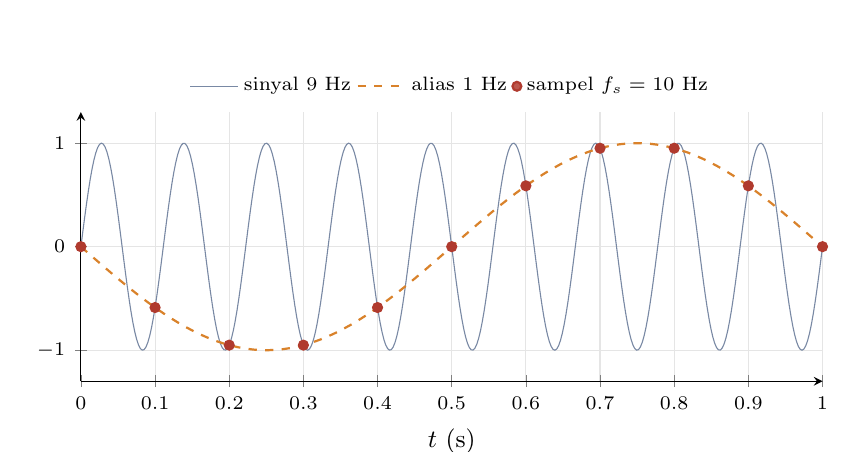
\begin{tikzpicture}
		\begin{axis}[skd,width=11cm,height=5cm,xmin=0,xmax=1,ymin=-1.3,ymax=1.3,xlabel={$t$ (s)},ytick={-1,0,1},legend style={at={(0.5,1.02)},anchor=south},legend columns=3]
			\addplot[skdblue!60,domain=0:1,samples=400,thin] {sin(deg(2*pi*9*x))};
			\addplot[skdorange,dashed,domain=0:1,samples=100] {-sin(deg(2*pi*x))};
			\addplot[skdred,only marks,mark=*,mark size=1.6pt,samples at={0,0.1,...,1}] {sin(deg(2*pi*9*x))};
			\legend{sinyal 9 Hz, alias 1 Hz, sampel $f_s=10$ Hz}
		\end{axis}
	\end{tikzpicture}
	\caption{\textit{Aliasing}: sinyal 9\,Hz dicacah 10\,Hz}
	\label{fig:b2-alias}
\end{figure}

\section{Rekonstruksi dengan \textit{data hold}}
\subsection{Zero-order hold}
DAC menahan setiap sampel konstan selama satu periode cacah: $u(t) = u(kT)$ untuk $kT \le t < (k+1)T$. Respons impuls ZOH adalah pulsa persegi selebar $T$, sehingga
\begin{equation}
	G_h(s) = \frac{1-e^{-sT}}{s},\qquad G_h(j\omega) = T\,\frac{\sin(\omega T/2)}{\omega T/2}\,e^{-j\omega T/2}.
\end{equation}
Penguatan ZOH pada frekuensi rendah adalah $T$, yang diimbangi faktor $1/T$ dari pencacah. Magnitudonya turun ke $2/\pi \approx 0{,}64$ di $\omega_N$, sehingga ZOH bukan filter rekonstruksi ideal. Yang paling penting untuk kontrol adalah fasanya, $-\omega T/2$: ZOH berperilaku seperti \textbf{tunda setengah waktu cacah}. Pendekatan praktisnya
\begin{equation}
	\frac{G_h(s)}{T} \approx e^{-sT/2} \approx \frac{1}{1+sT/2}.
\end{equation}

\subsection{First-order hold}
FOH mengekstrapolasi garis lurus dari dua sampel terakhir, $u(t) = u(kT) + \frac{u(kT)-u((k-1)T)}{T}(t-kT)$. Untuk sinyal yang mulus, batas galat rekonstruksinya $\frac{T^2}{2}\max|\ddot u|$, lebih kecil daripada ZOH ($T\max|\dot u|$), tetapi fasanya lebih buruk pada frekuensi tinggi dan implementasinya lebih rumit. DAC pada praktiknya selalu berupa ZOH.

\section{Memilih waktu cacah}
Waktu cacah yang terlalu besar menurunkan margin fasa (tunda $T/2$), memperlambat respons terhadap gangguan, dan berisiko \textit{aliasing}. Waktu cacah yang terlalu kecil membebani komputasi, membuat kutub diskrit menumpuk dekat $z=1$ sehingga peka terhadap kuantisasi koefisien (Bab~\ref{bab:impl}), dan membuat estimasi derivatif sangat berderau. Aturan praktis yang umum dipakai:
\begin{itemize}
	\item $\omega_s \approx 20$--$40$ kali \textit{bandwidth} kalang tertutup [FR 8.5];
	\item 4--10 sampel per waktu naik kalang tertutup;
	\item untuk plant FOPDT, $T \approx 0{,}1\tau$--$0{,}2\tau$ dan jauh lebih kecil dari tunda $\theta$.
\end{itemize}

\begin{contoh}[Waktu cacah untuk kontrol kecepatan motor]
	Plant $G_v(s) = 1/(0{,}5s+1)$ dengan target konstanta waktu kalang tertutup $\tau_{cl} \approx 0{,}15$\,s. \textit{Bandwidth} $\omega_b \approx 1/\tau_{cl} \approx 6{,}7$ rad/s, sehingga $\omega_s \approx 133$--$267$ rad/s atau $T \approx 0{,}024$--$0{,}047$\,s. Waktu naik $t_r \approx 2{,}2\tau_{cl} = 0{,}33$\,s; 4--10 sampel per waktu naik memberi $T \approx 0{,}03$--$0{,}08$\,s. Pilihan $T$ di kisaran 0,03--0,05\,s wajar. Contoh analitik di catatan ini memakai $T = 0{,}1$\,s agar angka mudah diikuti, dan dampaknya dianalisis di Bab~\ref{bab:responsz}--\ref{bab:stabil}. Selain itu waktu eksekusi \texttt{loop()} dan pengiriman serial harus jauh di bawah $T$.
\end{contoh}

\begin{ringkasan}
	Kuantisasi: $Q = \text{FSR}/2^n$, $\sigma_q^2 = Q^2/12$. Pencacahan membuat spektrum periodik dengan periode $\omega_s$; Shannon mensyaratkan $\omega_s > 2\omega_m$, jika tidak terjadi \textit{aliasing} yang harus dicegah dengan filter analog sebelum ADC. ZOH: $G_h(s) = (1-e^{-sT})/s$, setara tunda $T/2$. Waktu cacah dipilih dari \textit{bandwidth} atau waktu naik kalang tertutup.\\[3pt]
	\en{Quantisation step and noise; periodic spectrum of sampled signals; Shannon's theorem and aliasing; the ZOH behaves like a half-sample delay; choose $T$ from closed-loop bandwidth or rise time.}
\end{ringkasan}

\paragraph{Istilah kunci.} pencacahan \en{(sampling)}, kuantisasi \en{(quantisation)}, frekuensi Nyquist, filter \textit{anti-alias}, \textit{zero-order hold}, \textit{first-order hold}, rekonstruksi \en{(reconstruction)}, \textit{bandwidth}.

\section*{Latihan}
\begin{enumerate}
	\item Hitung $Q$ dan $\sigma_q$ untuk ADC 12-bit dengan rentang $\pm10$\,V.
	\item Sinyal 47\,Hz dicacah 40\,Hz. Berapa frekuensi aliasnya? Bagaimana dengan 130\,Hz yang dicacah 100\,Hz?
	\item Turunkan $G_h(j\omega)$ dari $G_h(s)$ dan tunjukkan bahwa fasanya $-\omega T/2$.
	\item Untuk $G(s) = 1/(0{,}2s+1)$ dengan target $\tau_{cl} = 0{,}05$\,s, usulkan $T$ dengan dua aturan praktis yang berbeda.
	\item Simulasikan sinus 9\,Hz yang dicacah 10\,Hz dengan MATLAB atau Python dan tampilkan aliasnya.
	\item Bandingkan konstanta waktu filter tachometer kit ($0{,}1$\,s) dengan waktu cacah 100\,ms. Apa konsekuensinya bagi identifikasi model kecepatan?
\end{enumerate}

\chapter{Persamaan Beda dan Transformasi Z}
\label{bab:z}
\enchap{Difference Equations and the Z-Transform}

\begin{tujuan}
	Setelah mempelajari bab ini, Anda mampu menulis model sistem diskrit sebagai persamaan beda, menghitung transformasi Z sinyal dasar, memakai sifat-sifatnya, menghitung transformasi Z invers, menyelesaikan persamaan beda, dan menghitung nilai akhir.
\end{tujuan}

\section{Persamaan beda}
Kontroler digital menjalankan \term{persamaan beda}{difference equation}: aturan rekursif yang menghitung keluaran baru dari keluaran lama dan masukan. Bentuk umum persamaan beda linier orde $n$ adalah
\begin{equation}
	y[k] + a_1y[k-1] + \dots + a_ny[k-n] = b_0u[k] + b_1u[k-1] + \dots + b_mu[k-m].
\end{equation}
Persamaan beda dapat diperoleh dengan mendekati turunan. Untuk plant kecepatan $\tau\dot y + y = Ku$, beda maju $\dot y(kT) \approx (y[k+1]-y[k])/T$ memberi
\begin{equation}
	y[k+1] = \Big(1 - \frac{T}{\tau}\Big)y[k] + \frac{KT}{\tau}u[k].
\end{equation}
Dengan $T=0{,}1$\,s, $\tau=0{,}5$\,s, dan $K=1$, diperoleh $y[k+1] = 0{,}8y[k] + 0{,}2u[k]$. Pendekatan Euler ini hanya aproksimasi; ekuivalen eksak dengan ZOH (Bab~\ref{bab:ftpulsa}) memberi koefisien $0{,}8187$ dan $0{,}1813$.

Persamaan beda dapat diselesaikan dengan rekursi. Untuk $y[k] = 0{,}8y[k-1] + 0{,}2u[k-1]$ dengan $y[0]=0$ dan $u[k]=1$, diperoleh $y = 0;\ 0{,}2;\ 0{,}36;\ 0{,}488;\ 0{,}590;\ \dots$ Rekursi mudah bagi komputer, tetapi tidak langsung memberi bentuk tertutup, nilai akhir, atau informasi kestabilan. Untuk itu diperlukan transformasi Z.

\section{Definisi transformasi Z}
Transformasi Z satu sisi barisan $x[k]$ didefinisikan sebagai
\begin{equation}
	X(z) = \mathcal{Z}\{x[k]\} = \sum_{k=0}^{\infty}x[k]\,z^{-k},
\end{equation}
dengan $z$ variabel kompleks dan deret konvergen untuk $|z| > R$ (\term{daerah konvergensi}{region of convergence}). Faktor $z^{-1}$ dapat dibaca sebagai operator tunda satu cacah. Hubungannya dengan Laplace sinyal tercacah adalah $z = e^{sT}$.

\begin{contoh}[Deret geometri]
	Untuk $x[k] = a^k$,
	\[
		X(z) = \sum_{k=0}^{\infty}(az^{-1})^k = \frac{1}{1-az^{-1}} = \frac{z}{z-a},\qquad |z| > |a|.
	\]
	Kasus khusus $a = 1$ memberi transformasi tangga satuan $z/(z-1)$, dan $a = e^{-\alpha T}$ memberi transformasi $e^{-\alpha t}$ yang dicacah.
\end{contoh}

Tabel~\ref{tab:b3-z} merangkum pasangan yang paling sering dipakai.

\begin{table}[H]
	\centering
	\caption{Pasangan transformasi Z}
	\label{tab:b3-z}
	\renewcommand{\arraystretch}{2.1}
	\begin{tabular}{@{}l l @{\qquad} l l@{}}
		\toprule
		$x[k]$ & $X(z)$ & $x(t)$ dicacah & $X(z)$ \\
		\midrule
		$\delta[k]$ & $1$ & $e^{-\alpha t}$ & $\dfrac{z}{z-e^{-\alpha T}}$ \\
		$1[k]$ & $\dfrac{z}{z-1}$ & $t$ & $\dfrac{Tz}{(z-1)^2}$ \\
		$k$ & $\dfrac{z}{(z-1)^2}$ & $\sin\omega t$ & $\dfrac{z\sin\omega T}{z^2-2z\cos\omega T+1}$ \\
		$a^k$ & $\dfrac{z}{z-a}$ & $\cos\omega t$ & $\dfrac{z(z-\cos\omega T)}{z^2-2z\cos\omega T+1}$ \\
		$ka^k$ & $\dfrac{az}{(z-a)^2}$ & $r^k\sin\theta k$ & $\dfrac{rz\sin\theta}{z^2-2rz\cos\theta+r^2}$ \\
		\bottomrule
	\end{tabular}
\end{table}

\section{Sifat-sifat}
Sifat-sifat berikut menjadikan transformasi Z alat yang efektif untuk menyelesaikan persamaan beda.
\begin{itemize}
	\item \textbf{Linieritas}: $\mathcal{Z}\{\alpha x[k] + \beta y[k]\} = \alpha X(z) + \beta Y(z)$.
	\item \textbf{Tunda}: $\mathcal{Z}\{x[k-n]\} = z^{-n}X(z)$ bila $x[k] = 0$ untuk $k < 0$.
	\item \textbf{Maju}: $\mathcal{Z}\{x[k+1]\} = zX(z) - zx[0]$ dan $\mathcal{Z}\{x[k+2]\} = z^2X(z) - z^2x[0] - zx[1]$. Kondisi awal masuk melalui sifat ini.
	\item \textbf{Skala}: $\mathcal{Z}\{a^kx[k]\} = X(z/a)$.
	\item \textbf{Diferensiasi}: $\mathcal{Z}\{kx[k]\} = -z\frac{d}{dz}X(z)$.
	\item \textbf{Konvolusi}: $\mathcal{Z}\big\{\sum_{j=0}^{k}x[j]y[k-j]\big\} = X(z)Y(z)$.
	\item \textbf{Nilai awal}: $x[0] = \lim_{z\to\infty}X(z)$.
	\item \textbf{Nilai akhir}: $\lim_{k\to\infty}x[k] = \lim_{z\to1}(z-1)X(z)$, \emph{hanya} bila semua kutub $(z-1)X(z)$ berada di dalam lingkaran satuan.
\end{itemize}

\begin{contoh}[Fungsi transfer dari persamaan beda]
	Transformasi kedua ruas $y[k] = 0{,}8y[k-1] + 0{,}2u[k-1]$ dengan kondisi awal nol memberi $Y(z)(1 - 0{,}8z^{-1}) = 0{,}2z^{-1}U(z)$, sehingga
	\[
		\frac{Y(z)}{U(z)} = \frac{0{,}2}{z-0{,}8}.
	\]
	Untuk masukan tangga, $Y(z) = \dfrac{0{,}2z}{(z-0{,}8)(z-1)}$ dan nilai akhirnya $\lim_{z\to1}(z-1)Y(z) = 0{,}2/0{,}2 = 1$, sama dengan penguatan DC plant. Pecahan parsial $Y(z)/z = \frac{1}{z-1} - \frac{1}{z-0{,}8}$ memberi bentuk tertutup $y[k] = 1 - 0{,}8^k$.
\end{contoh}

\section{Transformasi Z invers}
Ada tiga cara menghitung invers. \textbf{Pembagian panjang} membagi pembilang dengan penyebut dalam pangkat $z^{-1}$; koefisien $z^{-k}$ adalah $x[k]$. Cara ini cepat untuk beberapa sampel awal tetapi tidak memberi bentuk tertutup. \textbf{Pecahan parsial} menguraikan $X(z)/z$ menjadi suku-suku sederhana, mengalikannya kembali dengan $z$, lalu memakai tabel. Yang diuraikan adalah $X(z)/z$ karena tabel berbentuk $z/(z-a)$. \textbf{Integral inversi} memakai teorema residu, $x[k] = \sum\text{Res}[X(z)z^{k-1}]$, dan berguna untuk kutub berulang serta pembuktian.

\begin{contoh}[Persamaan beda orde dua]
	Selesaikan $y[k+2] - 0{,}7y[k+1] + 0{,}1y[k] = u[k]$ dengan kondisi awal nol dan $u$ tangga satuan.

	\textit{Transformasi.} $(z^2 - 0{,}7z + 0{,}1)Y(z) = \dfrac{z}{z-1}$, dan karena $z^2 - 0{,}7z + 0{,}1 = (z-0{,}5)(z-0{,}2)$,
	\[
		Y(z) = \frac{z}{(z-1)(z-0{,}5)(z-0{,}2)}.
	\]
	\textit{Pecahan parsial.} $\dfrac{Y(z)}{z} = \dfrac{c_1}{z-1} + \dfrac{c_2}{z-0{,}5} + \dfrac{c_3}{z-0{,}2}$ dengan
	\[
		c_1 = \frac{1}{(0{,}5)(0{,}8)} = \frac52,\quad c_2 = \frac{1}{(-0{,}5)(0{,}3)} = -\frac{20}{3},\quad c_3 = \frac{1}{(-0{,}8)(-0{,}3)} = \frac{25}{6}.
	\]
	\textit{Invers.}
	\[
		y[k] = \frac52 - \frac{20}{3}(0{,}5)^k + \frac{25}{6}(0{,}2)^k.
	\]
	Rumus ini memberi $y = 0;\ 0;\ 1;\ 1{,}7;\ 2{,}09;\ 2{,}293;\ \dots$, sama persis dengan rekursi $y[k+2] = 0{,}7y[k+1] - 0{,}1y[k] + 1$. Nilai akhirnya $c_1 = 2{,}5$, sesuai teorema nilai akhir $\lim_{z\to1}(z-1)Y(z) = 1/(0{,}5 \cdot 0{,}8)$.

	\textit{Pembagian panjang.} Dalam $z^{-1}$, $Y(z) = z^{-2}/(1 - 1{,}7z^{-1} + 0{,}8z^{-2} - 0{,}1z^{-3})$, dan pembagian memberi $z^{-2} + 1{,}7z^{-3} + 2{,}09z^{-4} + 2{,}293z^{-5} + \cdots$
\end{contoh}

\paragraph{Kutub kompleks dan berulang.} Pasangan kutub $z = re^{\pm j\theta}$ menghasilkan suku $Ar^k\cos(\theta k + \phi)$; pasangan sekawan digabung atau memakai baris terakhir Tabel~\ref{tab:b3-z}. Kutub berulang $(z-a)^2$ menghasilkan suku $ka^k$, dengan koefisien
\[
	c_{11} = \big[(z-a)^2X(z)/z\big]_{z=a},\qquad c_{12} = \frac{d}{dz}\big[(z-a)^2X(z)/z\big]_{z=a}.
\]
Secara umum, lokasi kutub menentukan bentuk respons: $|a| < 1$ meluruh, $|a| > 1$ membesar, dan $a < 0$ bergantian tanda. Hal ini dibahas lebih lanjut di Bab~\ref{bab:responsz}.

\begin{catatan}
	Perangkat lunak berguna untuk memeriksa hitungan tangan. Di MATLAB: \texttt{iztrans}, \texttt{residue}, dan \texttt{tf(num,den,T)} dengan \texttt{step}. Di Python: \texttt{sympy.apart(Y/z, z)} dan \texttt{control.tf(num, den, T)}.
\end{catatan}

\begin{ringkasan}
	Persamaan beda adalah model yang dieksekusi kontroler digital. $X(z) = \sum x[k]z^{-k}$ dan $z^{-1}$ berarti tunda satu cacah. Invers dihitung dengan menguraikan $X(z)/z$ menjadi pecahan parsial. Nilai akhir adalah $\lim_{z\to1}(z-1)X(z)$ bila sistem stabil.\\[3pt]
	\en{Difference equations are what digital controllers execute. The Z-transform turns them into algebra; partial fractions of $X(z)/z$ give closed-form solutions; the final value theorem applies only to stable signals.}
\end{ringkasan}

\paragraph{Istilah kunci.} persamaan beda \en{(difference equation)}, transformasi Z \en{(Z-transform)}, daerah konvergensi \en{(region of convergence)}, pecahan parsial \en{(partial fractions)}, pembagian panjang \en{(long division)}, teorema nilai akhir \en{(final value theorem)}.

\section*{Latihan}
\begin{enumerate}
	\item Tentukan $\mathcal{Z}\{k(0{,}5)^k\}$ dengan sifat diferensiasi dan periksa dengan Tabel~\ref{tab:b3-z}.
	\item Selesaikan $y[k] - 1{,}2y[k-1] + 0{,}32y[k-2] = u[k-1]$ untuk masukan impuls dengan kondisi awal nol.
	\item Hitung invers $X(z) = \dfrac{z^2}{(z-1)(z-0{,}6)}$ dan nilai akhirnya.
	\item Mengapa teorema nilai akhir tidak berlaku untuk $X(z) = z/(z-1{,}2)$?
	\item Selesaikan $y[k+1] - 0{,}5y[k] = 1$ dengan $y[0] = 2$ menggunakan sifat maju.
	\item Tentukan invers $X(z) = \dfrac{z}{z^2 - z + 0{,}5}$ dan nyatakan hasilnya dalam bentuk $Ar^k\sin(\theta k)$.
\end{enumerate}

\chapter{Fungsi Transfer Pulsa dan Identifikasi Model}
\label{bab:ftpulsa}
\enchap{Pulse Transfer Function and Model Identification}

\begin{tujuan}
	Setelah mempelajari bab ini, Anda mampu menurunkan fungsi transfer pulsa sistem tercacah dengan ZOH, menyusun fungsi transfer pulsa kalang tertutup, serta mengidentifikasi model FOPDT dan model ARX dari data dan memvalidasinya.
\end{tujuan}

\section{Fungsi transfer pulsa}
Untuk sistem linier dengan masukan dan keluaran tercacah, \term{fungsi transfer pulsa}{pulse transfer function} didefinisikan sebagai
\begin{equation}
	G(z) = \frac{Y(z)}{U(z)}\Big|_{\text{KA nol}} = \mathcal{Z}\{g[k]\},
\end{equation}
dengan $g[k]$ respons impuls diskrit. Keluaran adalah konvolusi diskrit $y[k] = \sum_{j=0}^{k}g[j]u[k-j]$, yang di domain $z$ menjadi perkalian $Y(z) = G(z)U(z)$.

\paragraph{Letak pencacah.} Dalam diagram blok sistem tercacah, hasil reduksi bergantung pada letak pencacah. Bila ada pencacah di antara dua blok, $Y(z)/U(z) = G_1(z)G_2(z)$. Bila tidak ada, kedua blok harus ditransformasikan bersama: $Y(z)/U(z) = \overline{G_1G_2}(z) = \mathcal{Z}\{G_1(s)G_2(s)\}$. Secara umum $\overline{G_1G_2}(z) \neq G_1(z)G_2(z)$. Misalnya untuk $G_1 = G_2 = 1/(s+1)$, $G_1(z)G_2(z) = z^2/(z-e^{-T})^2$ sedangkan $\overline{G_1G_2}(z) = Te^{-T}z/(z-e^{-T})^2$.

\section{Ekuivalen ZOH}
Karena ZOH dan plant tidak dipisahkan pencacah, keduanya ditransformasikan bersama:
\begin{equation}
	G(z) = \mathcal{Z}\left\{\frac{1-e^{-sT}}{s}G(s)\right\} = (1-z^{-1})\,\mathcal{Z}\left\{\frac{G(s)}{s}\right\}.
	\label{eq:b4-zoh}
\end{equation}
Persamaan~\eqref{eq:b4-zoh} memberi nilai \emph{eksak} keluaran plant pada saat cacah untuk masukan yang konstan sepotong-sepotong; tidak ada aproksimasi. Langkah praktisnya: (1) hitung $G(s)/s$; (2) uraikan dalam pecahan parsial; (3) ganti setiap suku dengan transformasi Z-nya; (4) kalikan dengan $(z-1)/z$. Di MATLAB atau Python, perintahnya \texttt{c2d(G,T,'zoh')}.

\begin{contoh}[Plant kecepatan motor]
	Untuk $G_v(s) = K/(\tau s+1)$,
	\[
		\frac{G_v(s)}{s} = K\left[\frac1s - \frac{1}{s+1/\tau}\right]
		\ \Rightarrow\
		\mathcal{Z}\Big\{\frac{G_v}{s}\Big\} = K\left[\frac{z}{z-1} - \frac{z}{z-a}\right],\quad a = e^{-T/\tau}.
	\]
	Mengalikan dengan $(z-1)/z$:
	\[
		G_v(z) = \frac{K(1-a)}{z-a}.
	\]
	Dengan $K=1$, $\tau=0{,}5$\,s, $T=0{,}1$\,s: $a = e^{-0{,}2} = 0{,}8187$, $b = 1-a = 0{,}1813$, sehingga $G_v(z) = 0{,}1813/(z-0{,}8187)$. Bandingkan dengan aproksimasi Euler $0{,}2/(z-0{,}8)$. Kutub kontinu $s = -1/\tau$ dipetakan ke $z = e^{-T/\tau}$.
\end{contoh}

\begin{contoh}[Plant posisi motor]
	Untuk $G_p(s) = K/(s(\tau s+1))$,
	\[
		\frac{G_p(s)}{s} = K\left[\frac{1}{s^2} - \frac{\tau}{s} + \frac{\tau}{s+1/\tau}\right].
	\]
	Dengan tabel dan perkalian $(z-1)/z$ diperoleh
	\[
		G_p(z) = \frac{b_1z + b_0}{(z-1)(z-a)},\qquad b_1 = K(T - \tau + \tau a),\quad b_0 = K(\tau - \tau a - aT).
	\]
	Angka acuan: $G_p(z) = \dfrac{0{,}009365\,z + 0{,}008762}{(z-1)(z-0{,}8187)}$, dengan kutub $z = 1$ (integrator) dan $z = 0{,}8187$, serta zero $z = -0{,}9356$. Zero ini tidak ada pada $G_p(s)$; ia muncul akibat pencacahan dan disebut \term{\textit{sampling zero}}{sampling zero}. Zero di dekat $z = -1$ ini penting untuk perancangan \textit{deadbeat} (Bab~\ref{bab:frek}).
\end{contoh}

Beberapa pasangan berguna: integrator $K/s$ menjadi $KT/(z-1)$, dan tunda murni $e^{-\theta s}$ dengan $\theta = dT$ menjadi $z^{-d}$. Tunda yang bukan kelipatan $T$ ditangani dengan transformasi Z termodifikasi [OG 3.5].

\section{Kalang tertutup}
Untuk umpan balik satuan dengan kontroler diskrit $D(z)$ dan plant tercacah $G(z)$,
\begin{equation}
	\frac{Y(z)}{R(z)} = \frac{D(z)G(z)}{1 + D(z)G(z)},
\end{equation}
dengan persamaan karakteristik $1 + D(z)G(z) = 0$. Bila sensor $H(s)$ juga kontinu tanpa pencacah di antara plant dan sensor, gunakan $\overline{GH}(z)$ pada penyebut.

\section{Identifikasi model dari data}
Parameter fisik jarang diketahui akurat, sedangkan model dari data otomatis mencakup sensor, filter, driver, dan aktuator. Alur identifikasi adalah: merancang eksperimen, mengambil data, memilih struktur model, mengestimasi parameter, lalu memvalidasi. Pada kit (Modul 1), \textit{deadzone} motor dikompensasi lebih dahulu, perubahan tangga diberikan di sekitar titik operasi, dan kecepatan direkam dengan waktu cacah tetap. Filter tachometer ($\tau_f = 0{,}1$\,s) ikut teridentifikasi sebagai bagian dari plant.

\subsection{Model FOPDT dari respons tangga}
Untuk respons tangga berbentuk sigmoid, model FOPDT $Ke^{-\theta s}/(\tau s+1)$ dapat diperoleh dengan \textbf{metode dua titik} (Smith). Catat waktu ketika respons mencapai 28,3\% dan 63,2\% dari perubahan akhir, $t_{28}$ dan $t_{63}$, lalu
\begin{equation}
	K = \frac{\Delta y_\infty}{\Delta u},\qquad \tau = 1{,}5\,(t_{63} - t_{28}),\qquad \theta = t_{63} - \tau.
\end{equation}

\begin{contoh}[Metode dua titik]
	Untuk respons plant $2e^{-0{,}3s}/(1{,}5s+1)$, $t_{28} = 0{,}799$\,s dan $t_{63} = 1{,}800$\,s, sehingga $\tau = 1{,}5(1{,}001) = 1{,}501$\,s dan $\theta = 0{,}299$\,s. Nilai sebenarnya 1,5\,s dan 0,3\,s. Metode garis singgung Ziegler--Nichols lebih peka terhadap derau karena bergantung pada kemiringan.
\end{contoh}

\subsection{Model ARX dan kuadrat terkecil}
Untuk plant kecepatan, struktur model yang sesuai dengan ekuivalen ZOH adalah ARX orde satu
\begin{equation}
	y[k] = a\,y[k-1] + b\,u[k-1] + e[k].
\end{equation}
Dengan $N$ data, persamaan disusun sebagai $\mathbf{Y} = \boldsymbol\Phi\boldsymbol\theta + \mathbf{e}$, dengan baris ke-$k$ dari $\boldsymbol\Phi$ adalah $[y[k-1]\ \ u[k-1]]$ dan $\boldsymbol\theta = [a\ \ b]^\top$. Meminimalkan $J = \|\mathbf{Y} - \boldsymbol\Phi\boldsymbol\theta\|^2$ memberi persamaan normal
\begin{equation}
	\hat{\boldsymbol\theta} = (\boldsymbol\Phi^\top\boldsymbol\Phi)^{-1}\boldsymbol\Phi^\top\mathbf{Y}.
\end{equation}
Parameter kontinu diperoleh dari $\hat\tau = -T/\ln\hat a$ dan $\hat K = \hat b/(1-\hat a)$.

\begin{contoh}[Identifikasi ARX]
	Data sintetis dari plant acuan dengan derau pengukuran $\sigma = 0{,}02$, 120 sampel, dan masukan berupa enam tingkat berbeda (Gambar~\ref{fig:b4-arx}). Estimasi kuadrat terkecil memberi $\hat a = 0{,}8217$ dan $\hat b = 0{,}1787$ (nilai benar 0,8187 dan 0,1813), sehingga $\hat\tau = 0{,}509$\,s dan $\hat K = 1{,}002$. Kecocokan simulasi model terhadap data, $\textit{fit} = 100\big(1 - \|y-\hat y\|/\|y-\bar y\|\big)$, adalah 92,3\%.
\end{contoh}

\begin{figure}[H]
	\centering
	\begin{tikzpicture}
		\begin{axis}[skd,width=12cm,height=5.4cm,xmin=0,xmax=12,ymin=-0.1,ymax=1.15,xlabel={$t$ (s)},legend style={at={(0.5,1.02)},anchor=south},legend columns=3]
			\addplot[skdgray,const plot,thin] table[x=t,y=u] {\dat{p4_arx.dat}};
			\addplot[skdblue,only marks,mark=*,mark size=0.8pt] table[x=t,y=ym] {\dat{p4_arx.dat}};
			\addplot[skdorange] table[x=t,y=yh] {\dat{p4_arx.dat}};
			\legend{masukan $u$, data terukur, simulasi model ARX}
		\end{axis}
	\end{tikzpicture}
	\caption{Identifikasi ARX orde satu}
	\label{fig:b4-arx}
\end{figure}

\subsection{Validasi}
Model harus diuji pada data yang tidak dipakai untuk estimasi, dengan simulasi bebas (bukan prediksi satu langkah). Residu sebaiknya acak dan tidak berkorelasi dengan masukan, dan parameter dibandingkan di beberapa titik operasi. Jebakan umum adalah masukan yang kurang ``kaya'' (hanya satu tangga), nonlinieritas seperti \textit{deadzone} dan saturasi yang membuat model hanya berlaku lokal, derau berwarna yang membuat estimasi kuadrat terkecil bias, dan waktu cacah yang jauh lebih kecil dari $\tau$ sehingga $\hat a$ sangat dekat 1 dan peka derau.

\begin{ringkasan}
	$G(z) = (1-z^{-1})\mathcal{Z}\{G(s)/s\}$ eksak pada saat cacah. Kutub $s = p$ menjadi $z = e^{pT}$ dan zero baru dapat muncul. Kalang tertutup: $DG/(1+DG)$. Model dari data diperoleh dengan metode grafis (FOPDT) atau kuadrat terkecil (ARX), dan selalu divalidasi.\\[3pt]
	\en{The ZOH equivalent is exact at sampling instants; sampling maps poles by $z = e^{pT}$ and may introduce sampling zeros. Empirical models from step tests or least-squares ARX fitting must always be validated.}
\end{ringkasan}

\paragraph{Istilah kunci.} fungsi transfer pulsa \en{(pulse transfer function)}, ekuivalen ZOH \en{(ZOH equivalent)}, \textit{sampling zero}, identifikasi sistem \en{(system identification)}, kuadrat terkecil \en{(least squares)}, validasi \en{(validation)}.

\section*{Latihan}
\begin{enumerate}
	\item Turunkan $G_p(z)$ untuk $G_p(s) = K/(s(\tau s+1))$ dan periksa angka acuan.
	\item Tentukan ekuivalen ZOH dari $\dfrac{2}{(s+1)(s+3)}$ dengan $T = 0{,}2$\,s.
	\item Buktikan $\overline{G_1G_2}(z) \neq G_1(z)G_2(z)$ untuk $G_1 = G_2 = 1/(s+1)$.
	\item Tentukan ekuivalen ZOH dari $e^{-0{,}2s}/(0{,}5s+1)$ dengan $T = 0{,}1$\,s.
	\item Dengan data Modul 1, estimasi model ARX orde satu, laporkan $K$, $\tau$, dan \textit{fit}, lalu validasi dengan data lain.
	\item Mengapa estimasi $\hat a$ menjadi peka derau bila $T \ll \tau$?
\end{enumerate}

\chapter{Emulasi dan PID Diskrit}
\label{bab:emulasi}
\enchap{Emulation and Discrete PID Control}

\begin{tujuan}
	Setelah mempelajari bab ini, Anda mampu mendiskritisasi pengontrol kontinu dengan berbagai metode, menjelaskan distorsi frekuensi Tustin dan \textit{prewarping}, menurunkan PID diskrit bentuk posisi dan kecepatan, menerapkan \textit{anti-windup} dan filter derivatif, serta menala PID diskrit secara heuristik.
\end{tujuan}

\section{Perancangan dengan emulasi}
Emulasi berarti merancang pengontrol kontinu $C(s)$ dengan metode yang sudah dikenal, lalu mengubahnya menjadi pengontrol diskrit $D(z)$ dan memverifikasi hasilnya dengan model diskrit plant. Kelebihannya, seluruh pengalaman kontrol kontinu dapat dipakai. Kekurangannya, tunda ZOH $T/2$ diabaikan saat merancang $C(s)$, sehingga hasilnya hanya baik bila $T$ kecil ($\omega_s \gtrsim 20\omega_b$).

\section{Metode diskritisasi}
\subsection{Aproksimasi integrasi}
Integrator $1/s$ dapat diganti dengan aturan integrasi numerik, yang setara dengan substitusi $s$ sebagai fungsi $z$:
\begin{align}
	\text{Euler maju:}\quad & s \leftarrow \frac{z-1}{T}, \\
	\text{Euler mundur:}\quad & s \leftarrow \frac{z-1}{zT}, \\
	\text{Tustin (bilinear):}\quad & s \leftarrow \frac{2}{T}\,\frac{z-1}{z+1}.
\end{align}
Ketiganya memetakan setengah bidang kiri bidang $s$ secara berbeda. Euler maju memetakannya ke setengah bidang $\text{Re}\,z < 1$, sehingga $C(s)$ yang stabil dapat menjadi $D(z)$ yang tidak stabil (misalnya $s = -50$ dengan $T = 0{,}05$\,s dipetakan ke $z = -1{,}5$). Euler mundur memetakannya ke lingkaran berpusat $0{,}5$ berjari-jari $0{,}5$, selalu stabil tetapi cenderung terlalu teredam. Tustin memetakan setengah bidang kiri tepat ke dalam lingkaran satuan, sehingga paling banyak dipakai.

\subsection{Distorsi frekuensi dan \textit{prewarping}}
Substitusi $z = e^{j\omega_dT}$ ke Tustin menghasilkan hubungan frekuensi
\begin{equation}
	\omega_c = \frac{2}{T}\tan\frac{\omega_dT}{2}.
\end{equation}
Seluruh sumbu $j\omega_c$ dimampatkan ke $0 \le \omega_d < \omega_N$. Distorsi kecil bila $\omega_d \ll \omega_N$. Agar satu frekuensi kritis $\omega_1$ (misalnya \textit{crossover} atau frekuensi \textit{notch}) dipetakan tepat, gunakan \textit{prewarping}:
\begin{equation}
	s \leftarrow \frac{\omega_1}{\tan(\omega_1T/2)}\,\frac{z-1}{z+1}.
\end{equation}

\subsection{\textit{Matched pole-zero}}
Metode MPZ memetakan setiap kutub dan zero berhingga dengan $z = e^{sT}$, memetakan zero di tak hingga ke $z = -1$ (atau membiarkan satu tunda agar kausal-tegas), lalu menyamakan penguatan DC $D(1) = C(0)$.

\begin{contoh}[Diskritisasi kompensator \textit{lead}]
	$C(s) = 10(s+2)/(s+10)$ dengan $T = 0{,}05$\,s menghasilkan:
	\begin{center}
		\renewcommand{\arraystretch}{2.0}
		\begin{tabular}{@{}l l@{}}
			\toprule
			Metode & $D(z)$ \\
			\midrule
			Euler maju & $\dfrac{10z - 9}{z - 0{,}5}$ \\
			Euler mundur & $\dfrac{7{,}333z - 6{,}667}{z - 0{,}6667}$ \\
			Tustin & $\dfrac{8{,}4z - 7{,}6}{z - 0{,}6}$ \\
			MPZ & $8{,}269\,\dfrac{z - 0{,}9048}{z - 0{,}6065}$ \\
			\bottomrule
		\end{tabular}
	\end{center}
	Pada MPZ, zero $e^{-2T} = 0{,}9048$, kutub $e^{-10T} = 0{,}6065$, dan penguatan dari $D(1) = C(0) = 2$. Di bawah sekitar 5\,rad/s respons frekuensi keempatnya hampir sama; mendekati $\omega_N = 62{,}8$\,rad/s perbedaannya besar, terutama pada fasa. Tustin dan MPZ paling dekat dengan $C(s)$ di rentang kerja.
\end{contoh}

\section{PID diskrit}
\subsection{Bentuk posisi}
Dengan integral persegi mundur dan derivatif beda mundur, PID menjadi
\begin{equation}
	u[k] = K_p\Big[e[k] + \frac{T}{T_i}\sum_{j=0}^{k}e[j] + \frac{T_d}{T}\big(e[k]-e[k-1]\big)\Big],
\end{equation}
yang diimplementasikan secara rekursif dengan $I[k] = I[k-1] + \frac{K_pT}{T_i}e[k]$. Fungsi transfernya
\begin{equation}
	D(z) = K_p\left[1 + \frac{T}{T_i}\,\frac{z}{z-1} + \frac{T_d}{T}\,\frac{z-1}{z}\right].
\end{equation}
Integrator diskrit adalah kutub di $z = 1$. Perhatikan bahwa penguatan derivatif efektif $K_pT_d/T$ membesar bila $T$ kecil, sehingga derau ikut membesar.

\subsection{Bentuk kecepatan}
Mengurangkan $u[k-1]$ dari $u[k]$ menghasilkan bentuk inkremental
\begin{equation}
	\Delta u[k] = q_0e[k] + q_1e[k-1] + q_2e[k-2],
\end{equation}
\begin{equation}
	q_0 = K_p\Big(1 + \frac{T}{T_i} + \frac{T_d}{T}\Big),\qquad q_1 = -K_p\Big(1 + \frac{2T_d}{T}\Big),\qquad q_2 = K_p\frac{T_d}{T},
\end{equation}
dengan $u[k] = u[k-1] + \Delta u[k]$. Contoh: $K_p = 2$, $T_i = 0{,}5$\,s, $T_d = 0{,}05$\,s, $T = 0{,}1$\,s memberi $q_0 = 3{,}4$, $q_1 = -4{,}0$, $q_2 = 1{,}0$. Bentuk kecepatan tidak memiliki akumulator eksplisit, memudahkan transfer manual--otomatis tanpa lonjakan, dan \textit{anti-windup} cukup dilakukan dengan membatasi $u[k]$.

\subsection{PID praktis}
Implementasi PID yang andal memerlukan beberapa modifikasi.
\begin{enumerate}
	\item \textbf{Filter derivatif}. $T_ds \rightarrow T_ds/(1 + T_ds/N)$; dengan Euler mundur dan $T_f = T_d/N$,
	\[
		D_f[k] = \frac{T_fD_f[k-1] + T_d\big(y[k]-y[k-1]\big)}{T_f + T}.
	\]
	\item \textbf{Derivatif pada pengukuran}: gunakan $-y$ alih-alih $e$ agar perubahan tangga \textit{setpoint} tidak menimbulkan lonjakan.
	\item \textbf{Bobot \textit{setpoint}}: bagian proporsional memakai $\beta r - y$ dengan $0 \le \beta \le 1$.
	\item \textbf{\textit{Anti-windup}}. Saat aktuator jenuh, integrator terus menumpuk galat sehingga menimbulkan lewatan besar. \textit{Clamping} menghentikan integrasi bila $u$ jenuh dan galat mendorong lebih jenuh; \textit{back-calculation} menambahkan $\frac{T}{T_t}(u_{\text{sat}} - u)$ ke integrator.
	\item \textbf{Batas nilai dan laju} $u$ sesuai aktuator (kit: $-100$ hingga $100\%$).
\end{enumerate}

\begin{contoh}[\textit{Integrator windup}]
	Plant kecepatan acuan dikontrol PI dengan $K_p = 3$, $T_i = 0{,}15$\,s, $T = 0{,}1$\,s, aktuator jenuh pada $|u| \le 1{,}2$, dan $r = 1$. Tanpa \textit{anti-windup}, $M_p \approx 19{,}6\%$ dan $t_s \approx 3{,}2$\,s. Dengan \textit{clamping}, $M_p \approx 0{,}3\%$ dan $t_s \approx 1{,}0$\,s (Gambar~\ref{fig:b5-windup}).
\end{contoh}

\begin{figure}[H]
	\centering
	\begin{tikzpicture}
		\begin{groupplot}[group style={group size=2 by 1,horizontal sep=1.5cm},skd,width=7cm,height=4.6cm,xmin=0,xmax=6,xlabel={$t$ (s)}]
			\nextgroupplot[ylabel={$y$},ymin=0,ymax=1.3,legend style={at={(0.98,0.05)},anchor=south east}]
			\addplot[skdgray,dashed,thin,domain=0:6,forget plot] {1};
			\addplot[skdred,const plot] table[x=t,y=yn] {\dat{p5_windup.dat}};
			\addplot[skdblue,const plot] table[x=t,y=yc] {\dat{p5_windup.dat}};
			\legend{tanpa AW, \textit{clamping}}
			\nextgroupplot[ylabel={$u$},ymin=0,ymax=1.4]
			\addplot[skdred,const plot] table[x=t,y=un] {\dat{p5_windup.dat}};
			\addplot[skdblue,const plot] table[x=t,y=uc] {\dat{p5_windup.dat}};
		\end{groupplot}
	\end{tikzpicture}
	\caption{Pengaruh \textit{anti-windup} pada PI dengan aktuator jenuh}
	\label{fig:b5-windup}
\end{figure}

\begin{lstlisting}[language=C++,caption={PID diskrit dengan D pada pengukuran dan \textit{clamping}},label={lst:b5-pid}]
float pid(float r, float y) {        // dipanggil tiap T
  float e = r - y;
  float P = Kp * e;
  Df = (Tf*Df + Td*(y - yPrev)) / (Tf + T);
  float D = -Kp * Df;                // D pada y
  float v = P + I + D;
  float u = constrain(v, -100, 100);
  if (u == v || e*v < 0)             // clamping
    I += Kp * T / Ti * e;
  yPrev = y;
  return u;
}
\end{lstlisting}

\section{Penalaan heuristik PID diskrit}
Karena ZOH menambah tunda sekitar $T/2$, tabel Ziegler--Nichols dan Cohen--Coon dipakai dengan tunda terkoreksi
\begin{equation}
	\theta' = \theta + \frac{T}{2}.
\end{equation}

\begin{contoh}[Koreksi tunda ZOH]
	Untuk plant FOPDT Bab~1 dengan $T = 0{,}05$\,s, penalaan dengan $\theta = 0{,}3$\,s ($K_p = 3{,}00$, $T_i = 0{,}60$\,s) menghasilkan $M_p \approx 89\%$ dan respons belum masuk pita 2\% dalam 8\,s. Dengan $\theta' = 0{,}325$\,s ($K_p = 2{,}77$, $T_i = 0{,}65$\,s, $T_d = 0{,}163$\,s) diperoleh $M_p \approx 72\%$ dan $t_s \approx 6{,}0$\,s. Koreksi membantu, tetapi ZN tetap agresif sehingga penalaan halus tetap diperlukan.
\end{contoh}

Prosedur penalaan halus: mulai dari hasil tabel dengan $\theta'$; turunkan $K_p$ hingga lewatan sesuai spesifikasi; atur $T_i$ (kecilkan untuk menghilangkan galat lebih cepat, besarkan bila berosilasi); tambahkan $T_d$ secukupnya sambil memperhatikan derau pada $u$; uji perubahan \textit{setpoint} naik, turun, dan gangguan beban; catat $M_p$, $t_s$, $e_{ss}$, IAE, dan $u_{\max}$. Prosedur ini dipraktikkan pada Modul 2.

\begin{ringkasan}
	Emulasi: rancang $C(s)$, lalu diskritisasi dengan Tustin atau MPZ; valid bila $T$ kecil. Euler maju dapat menghasilkan $D(z)$ tidak stabil. PID diskrit tersedia dalam bentuk posisi dan kecepatan; filter derivatif, derivatif pada pengukuran, dan \textit{anti-windup} wajib dalam praktik. Untuk penalaan heuristik, tambahkan $T/2$ pada tunda plant.\\[3pt]
	\en{Emulation discretises a continuous design (Tustin or matched pole-zero preferred). Discrete PID comes in position and velocity forms; practical PID needs derivative filtering, derivative on measurement, and anti-windup. Add $T/2$ to the process delay when using tuning tables.}
\end{ringkasan}

\paragraph{Istilah kunci.} emulasi \en{(emulation)}, transformasi bilinear (Tustin), \textit{prewarping}, \textit{matched pole-zero}, bentuk posisi/kecepatan \en{(position/velocity form)}, \textit{integrator windup}, \textit{anti-windup}, penalaan halus \en{(fine tuning)}.

\section*{Latihan}
\begin{enumerate}
	\item Diskritisasi $C(s) = 5(s+1)/(s+20)$ dengan Tustin dan MPZ untuk $T = 0{,}02$\,s, lalu bandingkan respons frekuensinya.
	\item Turunkan $q_0$, $q_1$, $q_2$ bentuk kecepatan dari bentuk posisi.
	\item Tunjukkan bahwa Euler maju memetakan $s = -50$ ke luar lingkaran satuan bila $T = 0{,}05$\,s.
	\item Turunkan rumus \textit{prewarping} dan terapkan untuk filter \textit{notch} 50\,Hz dengan $T = 1$\,ms.
	\item Simulasikan PI pada plant kecepatan dengan saturasi $|u| \le 1{,}2$, dengan dan tanpa \textit{anti-windup}.
	\item Mengapa penguatan derivatif efektif membesar bila $T$ dikecilkan, dan bagaimana filter derivatif mengatasinya?
\end{enumerate}

\chapter{Analisis Respons di Bidang $z$}
\label{bab:responsz}
\enchap{Response Analysis in the $z$-Plane}

\begin{tujuan}
	Setelah mempelajari bab ini, Anda mampu memetakan bidang $s$ ke bidang $z$, menghubungkan lokasi kutub diskrit dengan bentuk respons, menerjemahkan spesifikasi menjadi daerah kutub, menghitung galat keadaan tunak dari tipe sistem, dan menghitung indeks kinerja integral dari data diskrit.
\end{tujuan}

\section{Pemetaan $z = e^{sT}$}
Kutub kontinu $s = \sigma + j\omega$ dipetakan ke kutub diskrit
\begin{equation}
	z = e^{sT} = e^{\sigma T}e^{j\omega T},\qquad |z| = e^{\sigma T},\quad \angle z = \omega T.
\end{equation}
Akibatnya sumbu $j\omega$ menjadi lingkaran satuan $|z| = 1$, setengah bidang kiri menjadi bagian dalam lingkaran satuan, $s = 0$ menjadi $z = 1$, garis $\sigma$ konstan menjadi lingkaran $|z| = e^{\sigma T}$, garis $\omega$ konstan menjadi garis radial bersudut $\omega T$, dan $\omega = \pm\omega_s/2$ menjadi sumbu riil negatif. Pemetaan ini banyak-ke-satu: $s$ dan $s + jn\omega_s$ menghasilkan $z$ yang sama, sehingga hanya jalur primer $|\omega| < \omega_s/2$ yang bermakna. Contoh dengan $T = 0{,}1$\,s: $s = -2$ menjadi $z = 0{,}819$; $s = -20$ menjadi $z = 0{,}135$ (kutub cepat dekat titik asal); $s = -2 \pm j3{,}46$ menjadi $z = 0{,}819\angle\pm19{,}8^\circ$.

Untuk kutub orde dua $s = -\zeta\omega_n \pm j\omega_n\sqrt{1-\zeta^2}$,
\begin{equation}
	z = e^{-\zeta\omega_nT}\angle\pm\omega_nT\sqrt{1-\zeta^2}.
\end{equation}
Kurva $\zeta$ konstan adalah spiral logaritmik yang berawal di $z = 1$, dan kurva $\omega_nT$ konstan memotongnya (Gambar~\ref{fig:b6-kontur}). Sebaliknya, dari kutub diskrit $z = re^{\pm j\theta}$:
\begin{equation}
	\zeta = \frac{-\ln r}{\sqrt{\ln^2r + \theta^2}},\qquad \omega_n = \frac{\sqrt{\ln^2r + \theta^2}}{T}.
	\label{eq:b6-inv}
\end{equation}
Misalnya kutub $z = 0{,}6 \pm j0{,}3$ dengan $T = 0{,}1$\,s memberi $r = 0{,}671$, $\theta = 0{,}464$ rad, sehingga $\zeta = 0{,}65$ dan $\omega_n = 6{,}12$ rad/s.

\begin{figure}[H]
	\centering
	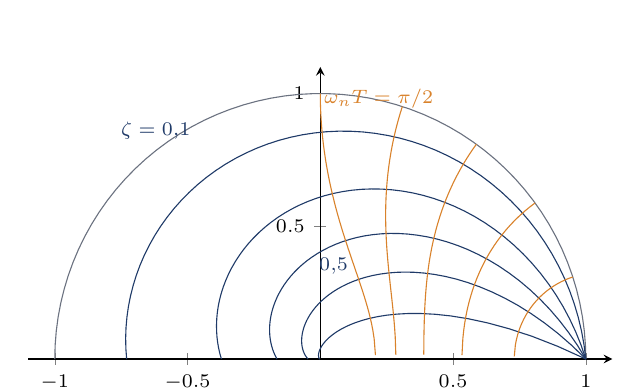
\begin{tikzpicture}
		\begin{axis}[width=9cm,height=9cm,axis equal image,xmin=-1.1,xmax=1.1,ymin=0,ymax=1.1,axis lines=middle,xtick={-1,-0.5,0.5,1},ytick={0.5,1},tick label style={font=\scriptsize}]
			\addplot[skdgray,domain=0:180,samples=60] ({cos(x)},{sin(x)});
			\foreach \zt in {0.1,0.3,0.5,0.7,0.9} {
					\addplot[skdblue,domain=0:3.14159,samples=60,variable=\t] ({exp(-\zt*\t/sqrt(1-\zt^2))*cos(deg(\t))},{exp(-\zt*\t/sqrt(1-\zt^2))*sin(deg(\t))});
				}
			\foreach \wn in {0.31416,0.62832,0.94248,1.25664,1.5708} {
					\addplot[skdorange,domain=0:0.999,samples=40,variable=\zz] ({exp(-\zz*\wn)*cos(deg(\wn*sqrt(1-\zz^2)))},{exp(-\zz*\wn)*sin(deg(\wn*sqrt(1-\zz^2)))});
				}
			\node[font=\scriptsize,text=skdblue] at (axis cs:-0.62,0.86) {$\zeta=0{,}1$};
			\node[font=\scriptsize,text=skdblue] at (axis cs:0.05,0.35) {$0{,}5$};
			\node[font=\scriptsize,text=skdorange] at (axis cs:0.22,0.98) {$\omega_nT=\pi/2$};
		\end{axis}
	\end{tikzpicture}
	\caption{Kontur $\zeta$ konstan (biru) dan $\omega_nT$ konstan (jingga) di bidang $z$}
	\label{fig:b6-kontur}
\end{figure}

\section{Lokasi kutub dan bentuk respons}
Kutub $z = re^{\pm j\theta}$ menghasilkan suku respons $r^k\cos(\theta k + \phi)$. Jari-jari $r$ menentukan laju peluruhan, sedangkan sudut $\theta$ menentukan jumlah sampel per periode osilasi, yaitu $2\pi/\theta$. Kutub riil positif dekat titik asal meluruh dalam beberapa cacah; kutub riil positif dekat $z = 1$ meluruh lambat; kutub riil negatif menghasilkan respons yang bergantian tanda setiap cacah (perilaku yang tidak punya padanan pada sistem kontinu orde satu); kutub di luar lingkaran satuan menghasilkan respons yang membesar. Kutub di $z = 0$ adalah tunda murni satu cacah.

\paragraph{Kutub dominan dan zero.} Kutub yang paling dekat dengan lingkaran satuan meluruh paling lambat dan disebut \term{kutub dominan}{dominant poles}. Rumus orde dua akurat bila kutub lain jauh lebih cepat (jari-jari jauh lebih kecil). Zero dekat $z = 1$ memperbesar lewatan, zero di sumbu riil negatif memengaruhi perilaku antar-cacah, dan pasangan kutub--zero yang berdekatan saling meniadakan tetapi dapat meninggalkan ekor lambat.

\section{Spesifikasi sebagai daerah kutub}
Spesifikasi kontinu diterjemahkan ke bidang $z$ sebagai berikut:
\begin{itemize}
	\item $t_s \approx 4/(\zeta\omega_n)$ memberi batas jari-jari $r \le e^{-4T/t_s}$;
	\item $M_p$ memberi batas $\zeta$, yaitu daerah di dalam spiral $\zeta$;
	\item batas $\omega_d$ (atau waktu puncak) memberi batas sudut.
\end{itemize}
Daerah yang diinginkan adalah irisan semuanya. Untuk $M_p \le 16\%$ ($\zeta \ge 0{,}5$) dan $t_s \le 2$\,s dengan $T = 0{,}1$\,s, batas jari-jarinya $e^{-0{,}2} = 0{,}819$; kutub $0{,}770 \pm j0{,}278$ berada tepat di batas dengan $\zeta = 0{,}50$ dan $\omega_n = 4{,}0$ rad/s. Daerah ini menjadi target perancangan di Bab~\ref{bab:rlocus} dan Bab~\ref{bab:pp}.

\begin{contoh}[Kontrol P kecepatan motor]
	Dengan $G_v(z) = b/(z-a)$ dan $D(z) = K_p$,
	\[
		\frac{Y(z)}{R(z)} = \frac{K_pb}{z - a + K_pb},\qquad z_{cl} = a - K_pb.
	\]
	Untuk $K_p = 2$: $z_{cl} = 0{,}8187 - 2(0{,}1813) = 0{,}4562$, setara dengan konstanta waktu $-T/\ln z_{cl} = 0{,}127$\,s (plant: 0,5\,s). Nilai akhir $K_pK/(1+K_pK) = 0{,}667$ dan galat tunak $1/(1+K_pK) = 0{,}333$. Bila $K_p > a/b = 4{,}52$, $z_{cl}$ menjadi negatif dan respons bergantian tanda.
\end{contoh}

\section{Galat keadaan tunak}
Untuk umpan balik satuan dengan $L(z) = D(z)G(z)$, galat adalah $E(z) = R(z)/(1+L(z))$ dan $e_{ss} = \lim_{z\to1}(z-1)E(z)$. \term{Tipe sistem}{system type} adalah jumlah kutub $L(z)$ di $z = 1$. Konstanta galat diskrit didefinisikan sebagai
\begin{equation}
	K_p = \lim_{z\to1}L(z),\qquad K_v = \lim_{z\to1}\frac{(z-1)L(z)}{T},\qquad K_a = \lim_{z\to1}\frac{(z-1)^2L(z)}{T^2},
\end{equation}
dengan $e_{ss} = 1/(1+K_p)$ untuk tangga, $1/K_v$ untuk \textit{ramp} $kT$, dan $1/K_a$ untuk parabola. Untuk plant posisi dengan kontrol P (tipe 1), galat tangga nol; karena $(z-1)G_p(z)|_{z=1} = (b_1+b_0)/(1-a) = 0{,}1 = KT$, diperoleh $K_v = K_pK$ dan $e_{ss}^{\text{ramp}} = 1/(K_pK)$. Hasil ini sama dengan kasus kontinu karena ekuivalen ZOH mempertahankan penguatan DC.

\section{Indeks kinerja integral}
Dari data diskrit dengan periode $T$, indeks kinerja dihitung sebagai
\begin{equation}
	\text{IAE} = T\sum_k|e[k]|,\qquad \text{ISE} = T\sum_ke[k]^2,\qquad \text{ITAE} = T^2\sum_kk\,|e[k]|.
\end{equation}
ISE menghukum galat besar di awal respons, ITAE menghukum galat yang bertahan lama, dan penambahan $\sum u[k]^2$ memasukkan usaha kontrol (dasar LQR di Bab~\ref{bab:lqr}). Dalam laporan praktikum, setiap uji sebaiknya dilaporkan dengan $t_r$, $t_s$ (2\%), $M_p$, $e_{ss}$, IAE, dan $u_{\max}$.

\begin{ringkasan}
	$z = e^{sT}$ memetakan setengah bidang kiri ke dalam lingkaran satuan. Jari-jari kutub menentukan peluruhan dan sudutnya menentukan frekuensi osilasi. Spesifikasi menjadi irisan lingkaran ($t_s$) dan spiral ($\zeta$). Tipe sistem adalah jumlah kutub di $z = 1$.\\[3pt]
	\en{The mapping $z = e^{sT}$ takes the left half-plane into the unit disc; pole radius sets decay, pole angle sets oscillation frequency; specifications become a region bounded by a circle and a $\zeta$-spiral; system type counts poles at $z = 1$.}
\end{ringkasan}

\paragraph{Istilah kunci.} bidang $z$ \en{($z$-plane)}, lingkaran satuan \en{(unit circle)}, kutub dominan \en{(dominant poles)}, tipe sistem \en{(system type)}, konstanta galat \en{(error constants)}, indeks kinerja \en{(performance index)}.

\section*{Latihan}
\begin{enumerate}
	\item Hitung $\zeta$ dan $\omega_n$ dari kutub $z = 0{,}6 \pm j0{,}3$ dengan $T = 0{,}1$\,s menggunakan Persamaan~\eqref{eq:b6-inv}.
	\item Gambarkan daerah kutub untuk $M_p \le 5\%$ dan $t_s \le 1$\,s dengan $T = 0{,}05$\,s.
	\item Untuk plant kecepatan dengan kontrol P, cari $K_p$ agar $e_{ss} \le 0{,}1$. Di mana kutubnya, dan bagaimana bentuk responsnya?
	\item Tunjukkan bahwa $(z-1)G_p(z)|_{z=1} = KT$.
	\item Hitung IAE, ISE, dan ITAE dari data respons Modul 1 atau 2.
\end{enumerate}

\chapter{Analisis Kestabilan Sistem Diskrit}
\label{bab:stabil}
\enchap{Stability Analysis of Discrete-Time Systems}

\begin{tujuan}
	Setelah mempelajari bab ini, Anda mampu menyatakan syarat kestabilan BIBO sistem diskrit, menerapkan uji Jury, menerapkan transformasi bilinear dengan kriteria Routh--Hurwitz, menghitung rentang penguatan stabil, dan menjelaskan pengaruh waktu cacah serta tunda komputasi terhadap kestabilan.
\end{tujuan}

\section{Syarat kestabilan}
Sistem dengan respons impuls $g[k]$ stabil BIBO jika dan hanya jika $\sum_{k=0}^{\infty}|g[k]| < \infty$. Untuk $G(z)$ rasional, setiap kutub $p_i$ menyumbang suku $c_ip_i^k$, sehingga
\begin{equation}
	\text{stabil} \iff |p_i| < 1 \ \text{untuk semua kutub}.
\end{equation}
Kutub sederhana pada $|z| = 1$ memberi kestabilan marginal (osilasi tetap atau integrator), sedangkan kutub di luar lingkaran satuan atau kutub berulang pada lingkaran satuan memberi ketidakstabilan. Untuk kalang tertutup, kutubnya adalah akar persamaan karakteristik $1 + D(z)G(z) = 0$.

\paragraph{Pencacahan dapat menggoyahkan kalang.} Plant kecepatan dengan kontrol P memiliki kutub kontinu $s = -(1+K_pK)/\tau$ yang stabil untuk semua $K_p > 0$. Versi diskritnya memiliki kutub $z_{cl} = a - K_pb$, yang stabil hanya bila $-1 < a - K_pb < 1$, yaitu
\begin{equation}
	0 < K_p < \frac{1+a}{K(1-a)} = \coth\frac{T}{2\tau}.
\end{equation}
Dengan $T = 0{,}1$\,s dan $\tau = 0{,}5$\,s, $K_{p,\max} = 10{,}03$. Penyebabnya adalah ZOH yang menahan aksi kontrol selama $T$: penguatan besar menghasilkan koreksi berlebih yang baru terlihat satu cacah kemudian.

\section{Uji Jury}
Untuk $P(z) = a_nz^n + \dots + a_1z + a_0$ dengan $a_n > 0$, \term{uji Jury}{Jury test} terdiri atas syarat perlu
\begin{equation}
	P(1) > 0,\qquad (-1)^nP(-1) > 0,\qquad |a_0| < a_n,
\end{equation}
dan, untuk $n \ge 3$, syarat tambahan dari tabel Jury. Baris pertama tabel adalah $a_0, a_1, \dots, a_n$ dan baris kedua kebalikannya. Baris berikutnya dihitung dengan
\begin{equation}
	b_k = \begin{vmatrix}a_0 & a_{n-k}\\ a_n & a_k\end{vmatrix} = a_0a_k - a_na_{n-k},\qquad k = 0, \dots, n-1,
\end{equation}
dengan syarat $|b_0| > |b_{n-1}|$, lalu proses diulang pada $b_k$ hingga baris terakhir berisi tiga elemen. Untuk orde dua, $P(z) = z^2 + a_1z + a_0$ stabil jika dan hanya jika $P(1) > 0$, $P(-1) > 0$, dan $|a_0| < 1$, yang di bidang $(a_1, a_0)$ membentuk segitiga dengan titik sudut $(-2,1)$, $(2,1)$, dan $(0,-1)$.

\begin{contoh}[Jury orde tiga]
	$P(z) = z^3 - 0{,}49z + 0{,}12$. Syarat perlu: $P(1) = 0{,}63 > 0$, $(-1)^3P(-1) = 0{,}39 > 0$, dan $|a_0| = 0{,}12 < 1$. Dengan $a_0 = 0{,}12$, $a_1 = -0{,}49$, $a_2 = 0$, $a_3 = 1$:
	\begin{align*}
		b_0 &= 0{,}12^2 - 1 = -0{,}9856, & b_1 &= (0{,}12)(-0{,}49) - 0 = -0{,}0588,\\
		b_2 &= 0 - (1)(-0{,}49) = 0{,}49. &&
	\end{align*}
	Karena $|b_0| = 0{,}9856 > |b_2| = 0{,}49$, sistem stabil. Pemeriksaan: akar $P(z)$ adalah $0{,}5$; $0{,}3$; dan $-0{,}8$.
\end{contoh}

\begin{contoh}[Rentang $K_p$ plant posisi]
	Dengan $G_p(z) = (b_1z+b_0)/((z-1)(z-a))$ dan $D(z) = K_p$, persamaan karakteristiknya
	\[
		z^2 + (K_pb_1 - 1 - a)z + (a + K_pb_0) = 0.
	\]
	Syarat Jury: $P(1) = K_p(b_1+b_0) > 0$ memberi $K_p > 0$; $P(-1) = 2(1+a) - K_p(b_1-b_0) > 0$ memberi $K_p < 6\,032$; dan $|a + K_pb_0| < 1$ memberi $K_p < (1-a)/b_0 = 20{,}69$. Jadi $0 < K_p < 20{,}69$. Pada batas itu kedua kutub kompleks berada tepat di lingkaran satuan. Versi kontinu stabil untuk semua $K_p > 0$.
\end{contoh}

\section{Transformasi bilinear dan Routh--Hurwitz}
Substitusi
\begin{equation}
	z = \frac{1+w}{1-w}\quad\Longleftrightarrow\quad w = \frac{z-1}{z+1}
\end{equation}
memetakan bagian dalam lingkaran satuan ke setengah bidang kiri bidang $w$. Setelah substitusi dan perkalian dengan $(1-w)^n$, kriteria Routh--Hurwitz diterapkan pada polinomial $w$; jumlah perubahan tanda kolom pertama tabel Routh sama dengan jumlah akar di luar lingkaran satuan.

\begin{contoh}[Tunda komputasi satu cacah]
	Bila aksi kontrol baru dikirim satu cacah setelah pengukuran, $L(z) = K_pb/(z(z-a))$ dan $P(z) = z^2 - az + K_pb$. Substitusi bilinear dan perkalian dengan $(1-w)^2$ menghasilkan
	\[
		(1 + a + K_pb)w^2 + 2(1 - K_pb)w + (1 - a + K_pb).
	\]
	Untuk orde dua, semua koefisien positif jika dan hanya jika $K_pb < 1$, sehingga $K_p < 1/b = 5{,}52$. Tunda satu cacah hampir memotong setengah penguatan maksimum ($10{,}03 \rightarrow 5{,}52$).
\end{contoh}

\section{Pengaruh waktu cacah dan tunda}
Gambar~\ref{fig:b7-kmax} menunjukkan $K_{p,\max}$ sebagai fungsi $T$ untuk ketiga kasus di atas. Bila $T \to 0$, $K_{p,\max} \to \infty$ dan kasus kontinu terpulihkan. Memperbesar $T$ menurunkan $K_{p,\max}$ dengan cepat, dan tunda komputasi menurunkannya lebih jauh.

\begin{figure}[H]
	\centering
	\begin{tikzpicture}
		\begin{axis}[skd,width=11cm,height=6cm,xmin=0,xmax=1,ymode=log,ymin=0.8,ymax=2000,xlabel={$T$ (s)},ylabel={$K_{p,\max}$},legend style={at={(0.98,0.98)},anchor=north east}]
			\addplot[skdblue] table[x=T,y=k1] {\dat{p7_kmax.dat}};
			\addplot[skdorange,dashed] table[x=T,y=k1d] {\dat{p7_kmax.dat}};
			\addplot[skdgreen] table[x=T,y=kpos] {\dat{p7_kmax.dat}};
			\legend{kecepatan + P, kecepatan + P + tunda, posisi + P}
		\end{axis}
	\end{tikzpicture}
	\caption{Penguatan maksimum yang stabil sebagai fungsi waktu cacah ($\tau = 0{,}5$\,s, $K=1$)}
	\label{fig:b7-kmax}
\end{figure}

Pemilihan metode uji bergantung pada keperluan: menghitung akar langsung paling praktis bila semua parameter numerik; Jury atau bilinear dengan Routh cocok untuk parameter simbolik seperti mencari rentang $K_p$ atau $T$; \textit{root locus} dan Nyquist (Bab~\ref{bab:rlocus}--\ref{bab:frek}) memperlihatkan bagaimana kutub bergerak dan seberapa besar margin. Perlu diingat bahwa kestabilan tidak sama dengan kinerja: kutub di $|z| = 0{,}98$ stabil, tetapi responsnya lambat dan berosilasi panjang.

\begin{ringkasan}
	Sistem diskrit stabil jika dan hanya jika semua kutub di dalam lingkaran satuan. Uji Jury: $P(1) > 0$, $(-1)^nP(-1) > 0$, $|a_0| < a_n$, ditambah tabel untuk $n \ge 3$. Transformasi bilinear dengan Routh adalah alternatif yang setara. Waktu cacah besar dan tunda komputasi menurunkan penguatan maksimum.\\[3pt]
	\en{A discrete system is stable iff all poles lie inside the unit circle; the Jury test and the bilinear transformation with Routh--Hurwitz give gain ranges symbolically; larger sampling periods and computation delays reduce the maximum stable gain.}
\end{ringkasan}

\paragraph{Istilah kunci.} kestabilan BIBO \en{(BIBO stability)}, persamaan karakteristik \en{(characteristic equation)}, uji Jury \en{(Jury test)}, transformasi bilinear \en{(bilinear transformation)}, stabil marginal \en{(marginally stable)}, tunda komputasi \en{(computational delay)}.

\section*{Latihan}
\begin{enumerate}
	\item Uji kestabilan $P(z) = z^3 - 1{,}2z^2 + 0{,}5z - 0{,}1$ dengan Jury.
	\item Tentukan rentang $K_p$ stabil untuk plant posisi dengan tunda komputasi satu cacah.
	\item Buktikan bahwa $(1+a)/(1-a) = \coth(T/2\tau)$ untuk $a = e^{-T/\tau}$.
	\item Untuk $K_p = 8$ pada plant kecepatan dengan $T = 0{,}1$\,s, hitung $z_{cl}$ dan sketsakan respons tangganya.
	\item Gunakan transformasi bilinear dan Routh untuk memeriksa soal nomor 1.
\end{enumerate}

\chapter{Perancangan dengan \textit{Root Locus} di Bidang $z$}
\label{bab:rlocus}
\enchap{Root-Locus Design in the $z$-Plane}

\begin{tujuan}
	Setelah mempelajari bab ini, Anda mampu menggambar dan membaca \textit{root locus} sistem diskrit, menerjemahkan spesifikasi menjadi kutub kalang tertutup yang diinginkan, merancang kompensator \textit{lead} diskrit dengan syarat sudut dan magnitudo, serta menambahkan aksi integral atau \textit{lag}.
\end{tujuan}

\section{\textit{Root locus} diskrit}
Persamaan karakteristik $1 + K\,L(z) = 0$ dipenuhi oleh titik-titik $z$ yang memenuhi
\begin{equation}
	\angle L(z) = \pm180^\circ(2q+1),\qquad K = \frac{1}{|L(z)|}.
\end{equation}
Aturan menggambarnya sama persis dengan bidang $s$: lokus berawal di kutub $L$ untuk $K = 0$ dan berakhir di zero untuk $K \to \infty$; pada sumbu riil, lokus berada di kiri jumlah ganjil kutub dan zero; asimtot, titik pisah, dan sudut keberangkatan dihitung dengan cara yang sama. Yang berbeda adalah interpretasinya. Batas stabil adalah lingkaran satuan, kontur kinerja adalah spiral $\zeta$ dan lingkaran $|z| = e^{-4T/t_s}$ (Bab~\ref{bab:responsz}), dan \textit{sampling zero} serta tunda ($z^{-d}$, kutub di $z = 0$) memengaruhi bentuk lokus.

\begin{contoh}[Plant posisi dengan kontrol P]
	$L(z) = G_p(z) = 0{,}009365(z + 0{,}9356)/((z-1)(z-0{,}8187))$. Kedua kutub bertemu di sumbu riil, lalu lokus melingkari zero $-0{,}936$ dan keluar dari lingkaran satuan pada $K_p = 20{,}7$, sesuai dengan uji Jury di Bab~\ref{bab:stabil}. Untuk $\zeta = 0{,}5$ diperlukan $K_p = 1{,}67$ dengan kutub $0{,}902 \pm j0{,}144$, yang memberi $M_p \approx 16\%$ tetapi $t_s \approx 4$\,s. Untuk respons yang lebih cepat diperlukan kompensator.
\end{contoh}

\section{Perancangan kompensator \textit{lead}}
Kompensator diskrit orde satu $D(z) = K_c(z - z_c)/(z - p_c)$ dirancang dengan langkah berikut.
\begin{enumerate}
	\item Dari spesifikasi, tentukan kutub kontinu $s_d = -\zeta\omega_n \pm j\omega_d$ dan petakan ke $z_d = e^{s_dT}$.
	\item Hitung $\angle G(z_d)$ dan defisit sudut $\phi = -180^\circ - \angle G(z_d)$ (modulo $360^\circ$).
	\item Pilih zero $z_c$, misalnya untuk membatalkan kutub plant yang lambat.
	\item Hitung kutub $p_c$ agar $\angle(z_d - z_c) - \angle(z_d - p_c) = \phi$.
	\item Hitung $K_c$ dari syarat magnitudo $|D(z_d)G(z_d)| = 1$.
	\item Verifikasi dengan simulasi, termasuk kutub lain dan respons antar-cacah.
\end{enumerate}

\begin{contoh}[\textit{Lead} untuk plant posisi]
	Spesifikasi: $\zeta = 0{,}5$, $t_s \le 2$\,s, $T = 0{,}1$\,s, dan galat tangga nol.

	\textit{Langkah 1.} $\zeta\omega_n = 4/t_s = 2$, $\omega_n = 4$, $\omega_d = 3{,}464$ rad/s, sehingga $z_d = e^{(-2+j3{,}464)(0{,}1)} = 0{,}819\angle19{,}85^\circ = 0{,}770 + j0{,}278$.

	\textit{Langkah 2.} $\angle G_p(z_d) = 139{,}74^\circ$, sehingga $\phi = -180^\circ - 139{,}74^\circ + 360^\circ = 40{,}26^\circ$.

	\textit{Langkah 3.} Zero membatalkan kutub plant: $z_c = 0{,}8187$, dengan $\angle(z_d - z_c) = 99{,}92^\circ$.

	\textit{Langkah 4.} $\angle(z_d - p_c) = 99{,}92^\circ - 40{,}26^\circ = 59{,}66^\circ$, sehingga $p_c = 0{,}770 - 0{,}278/\tan59{,}66^\circ = 0{,}607$.

	\textit{Langkah 5.} $K_c = 1/|G_p(z_d)(z_d - z_c)/(z_d - p_c)| = 7{,}18$.

	Hasilnya
	\[
		D(z) = 7{,}18\,\frac{z - 0{,}8187}{z - 0{,}6074},\qquad u[k] = 0{,}6074\,u[k-1] + 7{,}18\,e[k] - 5{,}877\,e[k-1].
	\]
	\textit{Langkah 6.} Kutub kalang tertutup $0{,}770 \pm j0{,}278$ (ditambah $0{,}8187$ yang dibatalkan zero). Simulasi memberi $M_p = 16{,}3\%$ dan $t_s = 2{,}1$\,s, dibandingkan $t_s = 4{,}0$\,s untuk kontrol P dengan redaman yang sama (Gambar~\ref{fig:b8-lead}). Aksi kontrol awal adalah $u[0] = K_c = 7{,}18$ untuk tangga satuan, sehingga kejenuhan aktuator perlu diperiksa. Lokus terkompensasi tetap stabil hingga $K_c \approx 45$, margin penguatan sekitar enam kali.
\end{contoh}

\begin{figure}[H]
	\centering
	\begin{tikzpicture}
		\begin{groupplot}[group style={group size=2 by 1,horizontal sep=1.5cm},skd,width=7cm,height=4.8cm,xmin=0,xmax=4,xlabel={$t$ (s)}]
			\nextgroupplot[ylabel={$y$},ymin=0,ymax=1.3,legend style={at={(0.98,0.05)},anchor=south east}]
			\addplot[skdgray,dashed,thin,domain=0:4,forget plot] {1};
			\addplot[skdblue,const plot] table[x=t,y=ylead] {\dat{p9_step.dat}};
			\addplot[skdorange,const plot] table[x=t,y=yp] {\dat{p9_step.dat}};
			\legend{\textit{lead}, P ($K_p=1{,}67$)}
			\nextgroupplot[ylabel={$u$ (\textit{lead})},ymin=-1,ymax=7.5]
			\addplot[skdblue,const plot] table[x=t,y=ulead] {\dat{p9_step.dat}};
		\end{groupplot}
	\end{tikzpicture}
	\caption{Respons tangga kontrol posisi dengan kompensator \textit{lead} diskrit}
	\label{fig:b8-lead}
\end{figure}

\begin{catatan}
	Pembatalan kutub--zero tidak pernah eksak pada perangkat keras; kutub $0{,}8187$ tetap ada sebagai pasangan kutub--zero yang hampir saling meniadakan. Ini aman karena kutub itu di dalam lingkaran satuan. Jangan pernah membatalkan kutub di luar atau pada lingkaran satuan: galat sekecil apa pun membuat kalang tertutup tidak stabil.
\end{catatan}

\section{Galat tunak: \textit{lag} dan PI diskrit}
Kompensator \textit{lag} $D_{\text{lag}}(z) = (z - z_l)/(z - p_l)$ dengan $p_l < z_l$ keduanya sangat dekat $z = 1$ menaikkan penguatan DC sebesar $(1-p_l)/(1-z_l)$ tanpa banyak mengubah sudut di $z_d$. PI diskrit adalah kasus $p_l = 1$, yang memberi galat tangga nol pada plant tipe 0. Untuk plant kecepatan, $D(z) = K_c(z - a)/(z-1)$ membatalkan kutub plant, sehingga $L(z) = K_cb/(z-1)$ dan kutub kalang tertutup $z = 1 - K_cb$ dapat ditala dengan satu parameter.

\section{Perancangan langsung atau emulasi}
Perancangan langsung di bidang $z$ memperhitungkan ZOH dan $T$ secara eksak dan tetap valid untuk $T$ relatif besar, tetapi memerlukan model $G(z)$ dan alat bidang $z$. Emulasi (Bab~\ref{bab:emulasi}) memanfaatkan intuisi kontinu tetapi kinerjanya turun bila $\omega_s < 20\omega_b$. Pada Modul 3, bandingkan PID hasil penalaan dengan kompensator \textit{lead} hasil \textit{root locus} dalam hal kinerja, usaha kontrol, dan ketahanan terhadap gangguan.

\begin{ringkasan}
	Aturan \textit{root locus} diskrit sama dengan kontinu, tetapi batas stabilnya lingkaran satuan. Spesifikasi diterjemahkan menjadi $z_d = e^{s_dT}$. Kompensator \textit{lead} dirancang dengan syarat sudut (untuk $p_c$) dan syarat magnitudo (untuk $K_c$); \textit{lag} atau PI ditambahkan untuk galat tunak. Jangan membatalkan kutub yang tidak stabil.\\[3pt]
	\en{Discrete root locus uses the same rules with the unit circle as stability boundary; design a lead compensator from angle and magnitude conditions at $z_d = e^{s_dT}$; add lag or PI action for steady-state error; never cancel unstable poles.}
\end{ringkasan}

\paragraph{Istilah kunci.} tempat kedudukan akar \en{(root locus)}, syarat sudut \en{(angle condition)}, syarat magnitudo \en{(magnitude condition)}, kompensator \textit{lead}/\textit{lag}, pembatalan kutub--zero \en{(pole--zero cancellation)}, defisit sudut \en{(angle deficiency)}.

\section*{Latihan}
\begin{enumerate}
	\item Ulangi perancangan \textit{lead} untuk $\zeta = 0{,}7$ dan $t_s = 1{,}5$\,s.
	\item Rancang PI diskrit untuk plant kecepatan agar $t_s = 0{,}6$\,s tanpa lewatan.
	\item Gambarkan lokus plant posisi dengan tunda komputasi $z^{-1}$ dan tentukan $K_{p,\max}$.
	\item Simulasikan rancangan nomor 1 dengan batas $|u| \le 1$ dan komentari hasilnya.
	\item Rancang \textit{lead} yang sama dengan memilih $z_c = 0{,}9$ (tanpa pembatalan) dan bandingkan responsnya.
\end{enumerate}

\chapter{Respons Frekuensi dan Perancangan Langsung}
\label{bab:frek}
\enchap{Frequency Response and Direct Design}

\begin{tujuan}
	Setelah mempelajari bab ini, Anda mampu menghitung respons frekuensi dan margin kestabilan sistem diskrit, menjelaskan pengaruh ZOH pada margin fasa, memakai transformasi $w$ untuk perancangan dengan diagram Bode, serta merancang pengontrol \textit{deadbeat} dan Dahlin dengan metode Ragazzini.
\end{tujuan}

\section{Respons frekuensi sistem diskrit}
Masukan sinusoidal $u[k] = \sin(\omega kT)$ pada sistem stabil $G(z)$ menghasilkan keluaran tunak
\begin{equation}
	y[k] = |G(e^{j\omega T})|\sin\big(\omega kT + \angle G(e^{j\omega T})\big).
\end{equation}
Respons frekuensi diperoleh dengan mengevaluasi $G(z)$ pada lingkaran satuan $z = e^{j\omega T}$. Respons ini periodik dengan periode $\omega_s$, sehingga cukup digambar hingga $\omega_N = \pi/T$. Margin penguatan (GM) dan margin fasa (PM) didefinisikan seperti pada sistem kontinu. Acuan praktik yang umum adalah PM $30^\circ$--$60^\circ$, GM $\ge 6$\,dB, dan puncak sensitivitas $M_s \le 2$; untuk PM di bawah $60^\circ$, redaman kalang tertutup kira-kira $\zeta \approx \text{PM}/100$.

\begin{contoh}[Pengaruh ZOH pada margin]
	Plant posisi dengan $K_p = 5$. Versi kontinu memiliki frekuensi \textit{crossover} 2,86 rad/s, PM $= 34{,}9^\circ$, dan GM tak hingga. Versi diskrit dengan $T = 0{,}1$\,s memiliki \textit{crossover} yang sama, tetapi PM $= 26{,}8^\circ$ dan GM $= 12{,}3$\,dB pada 6,22 rad/s. Selisih PM sekitar $\omega_cT/2 = 8{,}2^\circ$ adalah tunda setengah cacah dari ZOH, dan fasa yang terus turun menuju $\omega_N$ membuat GM menjadi berhingga.
\end{contoh}

\section{Transformasi $w$}
Transformasi
\begin{equation}
	w = \frac{2}{T}\,\frac{z-1}{z+1},\qquad z = \frac{1 + wT/2}{1 - wT/2}
\end{equation}
memetakan lingkaran satuan ke sumbu imajiner $w = j\nu$, dengan frekuensi semu $\nu = \frac{2}{T}\tan\frac{\omega T}{2}$. Fungsi $G(w)$ rasional sehingga seluruh alat Bode kontinu dapat dipakai. Di bawah sekitar $\omega_s/10$, $\nu \approx \omega$; dengan $T = 0{,}1$\,s, $\omega = 10$ rad/s menjadi $\nu = 10{,}9$, sedangkan $\omega = 30$ rad/s menjadi $\nu = 282$. Prosedur perancangannya: hitung $G(z)$ (ZOH) lalu $G(w)$; rancang $C(w)$ dengan Bode untuk PM dan GM target; substitusi $w = \frac2T\frac{z-1}{z+1}$ untuk memperoleh $D(z)$; verifikasi di domain waktu. Berbeda dari emulasi Tustin, ZOH sudah termasuk dalam $G(w)$ sehingga tidak ada aproksimasi.

\section{Perancangan langsung (Ragazzini)}
Dalam metode Ragazzini, fungsi transfer kalang tertutup yang diinginkan $F(z)$ ditentukan terlebih dahulu, lalu kontroler diselesaikan dari $F = DG/(1+DG)$:
\begin{equation}
	D(z) = \frac{1}{G(z)}\,\frac{F(z)}{1 - F(z)}.
\end{equation}
Karena kontroler ini ``membalik'' plant, $F(z)$ harus memenuhi tiga syarat:
\begin{enumerate}
	\item \textbf{Kausalitas}: tunda $F$ tidak boleh lebih kecil dari tunda $G$ (selisih derajat penyebut dan pembilang).
	\item \textbf{Kestabilan internal}: zero $G$ di luar atau dekat lingkaran satuan harus menjadi zero $F$, dan kutub $G$ yang tidak stabil harus menjadi zero $1-F$.
	\item \textbf{Galat tunak}: untuk masukan tangga, $F(1) = 1$, yaitu $1-F(z)$ mengandung faktor $(z-1)$.
\end{enumerate}

\begin{contoh}[\textit{Deadbeat} dan Dahlin pada plant kecepatan]
	$G_v(z) = b/(z-a)$ memiliki tunda satu cacah tanpa zero bermasalah. Pengontrol \textbf{\textit{deadbeat}} memilih $F(z) = z^{-1}$, sehingga keluaran tepat di \textit{setpoint} setelah satu cacah:
	\[
		D(z) = \frac{z-a}{b}\cdot\frac{z^{-1}}{1-z^{-1}} = \frac{z-a}{b(z-1)}.
	\]
	Ini adalah PI dengan zero yang membatalkan kutub plant. Aksi awalnya $u[0] = 1/b = 5{,}52$, lalu $u[k] = 1$. Pengontrol \textbf{Dahlin} memilih respons orde satu dengan konstanta waktu $\lambda$: $F(z) = (1-q)/(z-q)$ dengan $q = e^{-T/\lambda}$, sehingga
	\[
		D(z) = \frac{(1-q)(z-a)}{b(z-1)}.
	\]
	Dengan $\lambda = 0{,}3$\,s, $q = 0{,}7165$ dan $u[0] = (1-q)/b = 1{,}56$. Respons lebih lambat ($y = 0{,}28;\ 0{,}49;\ 0{,}63;\ \dots$) tetapi usaha kontrol jauh lebih kecil. Parameter $\lambda$ menjadi satu tombol penala antara kecepatan dan usaha kontrol.
\end{contoh}

\begin{contoh}[\textit{Deadbeat} plant posisi dan riak antar-cacah]
	Untuk plant posisi, pilihan \textit{minimal prototype} $F = z^{-1}$ menghasilkan $D(z)$ yang membatalkan \textit{sampling zero} $-0{,}936$. Sampel $y[k]$ memang mencapai 1 setelah satu cacah, tetapi aksi kontrol bergantian tanda dengan amplitudo ratusan dan keluaran kontinu $y(t)$ beriak di antara cacah (Gambar~\ref{fig:b9-ripple}). Desain \textbf{bebas riak} memasukkan zero plant ke dalam $F$:
	\[
		F(z) = \frac{b_1z + b_0}{(b_1+b_0)z^2},\qquad 1 - F(z) = (1 - z^{-1})(1 + cz^{-1}),\quad c = \frac{b_0}{b_1+b_0} = 0{,}483,
	\]
	sehingga $D(z) = \dfrac{1 - az^{-1}}{(b_1+b_0)(1 + cz^{-1})}$. Respons selesai dalam dua cacah dan $u$ konstan setelahnya, tetapi $u[0] = 55$ masih sangat besar karena $T$ kecil. \textit{Deadbeat} cocok bila $T$ besar atau aktuator kuat.
\end{contoh}

\begin{figure}[H]
	\centering
	\begin{tikzpicture}
		\begin{groupplot}[group style={group size=2 by 1,horizontal sep=1.5cm},skd,width=7cm,height=4.8cm,xmin=0,xmax=1.5,xlabel={$t$ (s)}]
			\nextgroupplot[ylabel={$y(t)$},ymin=0,ymax=1.5,legend style={at={(0.98,0.97)},anchor=north east}]
			\addplot[skdgray,dashed,thin,domain=0:1.5,forget plot] {1};
			\addplot[skdred] table[x=t,y=ymp] {\dat{p10_ripple.dat}};
			\addplot[skdblue] table[x=t,y=yrf] {\dat{p10_ripple.dat}};
			\legend{\textit{minimal prototype}, bebas riak}
			\nextgroupplot[ylabel={$u$},ymin=-200,ymax=200]
			\addplot[skdred] table[x=t,y=ump] {\dat{p10_ripple.dat}};
			\addplot[skdblue] table[x=t,y=urf] {\dat{p10_ripple.dat}};
		\end{groupplot}
	\end{tikzpicture}
	\caption{\textit{Deadbeat} plant posisi: riak antar-cacah dan desain bebas riak}
	\label{fig:b9-ripple}
\end{figure}

Perancangan langsung cocok untuk proses lambat dengan $T$ relatif besar, plant dengan tunda murni (Dahlin memberi bentuk respons yang dapat diprediksi), dan kasus dengan model akurat serta aktuator yang tidak mudah jenuh. Kelemahannya: pembatalan plant peka terhadap galat model, usaha kontrol besar bila $T$ kecil, respons hanya dijamin pada saat cacah, dan tidak ada jaminan margin kestabilan.

\begin{ringkasan}
	Respons frekuensi diskrit dievaluasi pada $z = e^{j\omega T}$ hingga $\omega_N$; ZOH mengurangi PM sekitar $\omega_cT/2$. Transformasi $w$ memungkinkan perancangan Bode untuk plant diskrit tanpa aproksimasi. Metode Ragazzini $D = \frac{1}{G}\frac{F}{1-F}$ memerlukan $F$ yang kausal, menjamin kestabilan internal, dan memenuhi galat tunak. \textit{Deadbeat} cepat tetapi mahal; Dahlin lebih lunak.\\[3pt]
	\en{Discrete frequency response and margins; the ZOH costs about $\omega_cT/2$ of phase margin; $w$-plane design applies Bode methods exactly; Ragazzini's method specifies the closed loop directly, with deadbeat and Dahlin as special cases.}
\end{ringkasan}

\paragraph{Istilah kunci.} respons frekuensi \en{(frequency response)}, margin fasa/penguatan \en{(phase/gain margin)}, transformasi $w$ \en{($w$-transformation)}, perancangan langsung \en{(direct design)}, \textit{deadbeat}, riak antar-cacah \en{(intersample ripple)}.

\section*{Latihan}
\begin{enumerate}
	\item Hitung $G_p(w)$ untuk plant posisi dan rancang \textit{lead} agar PM $= 50^\circ$.
	\item Rancang Dahlin untuk plant kecepatan dengan $\lambda = 0{,}2$\,s dan hitung $u[0]$.
	\item Turunkan $D(z)$ \textit{deadbeat} bebas riak untuk plant posisi dan periksa barisan $u[k]$.
	\item Ulangi \textit{deadbeat} plant posisi untuk $T = 0{,}5$\,s; bandingkan $u[0]$ dengan $T = 0{,}1$\,s.
	\item Jelaskan mengapa \textit{deadbeat} \textit{minimal prototype} menimbulkan riak bila $G(z)$ memiliki zero dekat $z = -1$.
\end{enumerate}

\chapter{Ruang Keadaan Diskrit}
\label{bab:ss}
\enchap{Discrete-Time State Space}

\begin{tujuan}
	Setelah mempelajari bab ini, Anda mampu menulis model ruang keadaan kontinu dan diskrit, mendiskritisasi model kontinu, menghitung solusi dan fungsi transfer pulsa dari ruang keadaan, menyusun bentuk kanonik, serta menguji keterkendalian dan keteramatan.
\end{tujuan}

\section{Model ruang keadaan}
Model ruang keadaan menggambarkan variabel internal sistem, alami untuk sistem banyak masukan--banyak keluaran, dan menjadi dasar perancangan modern: penempatan kutub, pengamat, LQR, filter Kalman, dan MPC. Bentuk kontinu dan diskritnya adalah
\begin{align}
	\dot{\mathbf{x}} &= A\mathbf{x} + B\mathbf{u}, & \mathbf{y} &= C\mathbf{x} + D\mathbf{u},\\
	\mathbf{x}[k+1] &= \Phi\mathbf{x}[k] + \Gamma\mathbf{u}[k], & \mathbf{y}[k] &= C\mathbf{x}[k] + D\mathbf{u}[k].
\end{align}

Untuk motor DC posisi, dari $\tau\dot\omega + \omega = Ku$ dan $\dot\theta = \omega$, pilih $\mathbf{x} = [\theta\ \ \omega]^\top$:
\begin{equation}
	A = \begin{bmatrix}0 & 1\\ 0 & -1/\tau\end{bmatrix},\qquad B = \begin{bmatrix}0\\ K/\tau\end{bmatrix},\qquad C = \begin{bmatrix}1 & 0\end{bmatrix}.
\end{equation}
Pada kit, $\theta$ diukur potensiometer dan $\omega$ diukur tachometer melalui filter. Model dua keadaan ini dipakai pada Modul 4.

\section{Diskritisasi dengan ZOH}
Solusi persamaan keadaan dari $kT$ ke $(k+1)T$ dengan $u$ konstan adalah
\begin{equation}
	\mathbf{x}((k+1)T) = e^{AT}\mathbf{x}(kT) + \int_0^Te^{A\eta}\,d\eta\,B\,u(kT),
\end{equation}
sehingga
\begin{equation}
	\Phi = e^{AT},\qquad \Gamma = \int_0^Te^{A\eta}\,d\eta\;B.
\end{equation}
Hasilnya eksak pada saat cacah, sama seperti ekuivalen ZOH fungsi transfer. Matriks eksponensial dapat dihitung dengan deret $I + AT + (AT)^2/2! + \cdots$, dengan Laplace $e^{AT} = \mathcal{L}^{-1}\{(sI-A)^{-1}\}|_{t=T}$, atau secara numerik dengan matriks diperbesar
\begin{equation}
	\exp\left(\begin{bmatrix}A & B\\ 0 & 0\end{bmatrix}T\right) = \begin{bmatrix}\Phi & \Gamma\\ 0 & I\end{bmatrix}.
\end{equation}

\begin{contoh}[Model diskrit motor posisi]
	Dengan $a = e^{-T/\tau}$, hasil analitiknya
	\[
		\Phi = \begin{bmatrix}1 & \tau(1-a)\\ 0 & a\end{bmatrix},\qquad \Gamma = \begin{bmatrix}K\big(T - \tau(1-a)\big)\\ K(1-a)\end{bmatrix}.
	\]
	Untuk $T = 0{,}1$\,s:
	\[
		\Phi = \begin{bmatrix}1 & 0{,}09063\\ 0 & 0{,}81873\end{bmatrix},\qquad \Gamma = \begin{bmatrix}0{,}00937\\ 0{,}18127\end{bmatrix}.
	\]
	Nilai eigen $\Phi$ adalah 1 dan 0,8187, sama dengan kutub $G_p(z)$; baris keduanya sama dengan $G_v(z)$ plant kecepatan.
\end{contoh}

\section{Solusi dan fungsi transfer}
Rekursi berulang memberi solusi
\begin{equation}
	\mathbf{x}[k] = \Phi^k\mathbf{x}[0] + \sum_{j=0}^{k-1}\Phi^{k-1-j}\Gamma u[j].
\end{equation}
Respons bebas ditentukan oleh nilai eigen $\Phi$: $\Phi^k \to 0$ bila semua $|\lambda_i| < 1$. Dengan kondisi awal nol, transformasi Z memberi
\begin{equation}
	G(z) = C(zI - \Phi)^{-1}\Gamma + D,
\end{equation}
dengan kutub akar $\det(zI - \Phi) = 0$. Untuk contoh motor,
\[
	(zI - \Phi)^{-1} = \frac{1}{(z-1)(z-a)}\begin{bmatrix}z-a & \tau(1-a)\\ 0 & z-1\end{bmatrix},\qquad
	C(zI-\Phi)^{-1}\Gamma = \frac{0{,}009365\,z + 0{,}008762}{z^2 - 1{,}8187z + 0{,}8187},
\]
sama dengan $G_p(z)$ dari Bab~\ref{bab:ftpulsa}.

\section{Bentuk kanonik dan transformasi similaritas}
Untuk $G(z) = (b_1z + b_0)/(z^2 + a_1z + a_0)$, bentuk kanonik keterkendalian adalah
\begin{equation}
	\Phi_c = \begin{bmatrix}0 & 1\\ -a_0 & -a_1\end{bmatrix},\quad \Gamma_c = \begin{bmatrix}0\\ 1\end{bmatrix},\quad C_c = \begin{bmatrix}b_0 & b_1\end{bmatrix},
\end{equation}
dan bentuk kanonik keteramatan adalah $\Phi_o = \Phi_c^\top$, $\Gamma_o = C_c^\top$, $C_o = \Gamma_c^\top$. Realisasi ruang keadaan tidak unik: perubahan koordinat $\mathbf{x} = P\bar{\mathbf{x}}$ memberi $\bar\Phi = P^{-1}\Phi P$, $\bar\Gamma = P^{-1}\Gamma$, $\bar C = CP$ dengan fungsi transfer yang sama. Bentuk kanonik memudahkan perhitungan, sedangkan keadaan fisik lebih bermakna untuk implementasi.

\section{Keterkendalian dan keteramatan}
Sistem \term{terkendali}{controllable} bila setiap keadaan awal dapat dibawa ke keadaan mana pun dalam $n$ langkah, dan \term{teramati}{observable} bila keadaan awal dapat ditentukan dari $n$ pengukuran keluaran dan masukan. Uji rank-nya:
\begin{equation}
	W_c = \begin{bmatrix}\Gamma & \Phi\Gamma & \cdots & \Phi^{n-1}\Gamma\end{bmatrix},\qquad
	W_o = \begin{bmatrix}C\\ C\Phi\\ \vdots\\ C\Phi^{n-1}\end{bmatrix},
\end{equation}
dengan syarat rank $W_c = n$ dan rank $W_o = n$. Keterkendalian diperlukan untuk menempatkan kutub sembarang, dan keteramatan diperlukan untuk pengamat keadaan.

\begin{contoh}[Motor posisi]
	$W_c = \begin{bmatrix}0{,}00937 & 0{,}02579\\ 0{,}18127 & 0{,}14841\end{bmatrix}$ dengan $\det W_c = -0{,}00329 \ne 0$, sehingga terkendali. Dengan pengukuran posisi $C = [1\ \ 0]$, $W_o = \begin{bmatrix}1 & 0\\ 1 & 0{,}09063\end{bmatrix}$ dengan determinan $0{,}0906$, sehingga teramati: kecepatan dapat diestimasi dari posisi. Dengan pengukuran kecepatan saja, $C = [0\ \ 1]$, $W_o = \begin{bmatrix}0 & 1\\ 0 & 0{,}8187\end{bmatrix}$ dengan determinan nol: posisi tidak dapat direkonstruksi dari kecepatan karena konstanta integrasinya tidak diketahui.
\end{contoh}

\paragraph{Pencacahan patologis.} Pencacahan dapat menghilangkan keterkendalian atau keteramatan. Untuk osilator $\ddot x + \omega_0^2x = u$ dengan $\omega_0 = 2\pi$ rad/s, $T = 0{,}4$\,s memberi $\det W_c = -8{,}6\times10^{-3}$ (terkendali), tetapi $T = 0{,}5$\,s (setengah periode) memberi $\Phi = -I$ dan $\det W_c = 0$. Secara umum, untuk mode osilasi $\sigma \pm j\omega_0$, keterkendalian atau keteramatan dapat hilang bila $\omega_0T = q\pi$, $q = 1, 2, \dots$, karena pencacah melihat osilasi pada fasa yang sama setiap kali.

\begin{ringkasan}
	$\Phi = e^{AT}$ dan $\Gamma = \int_0^Te^{A\eta}d\eta\,B$ eksak dengan ZOH. $G(z) = C(zI-\Phi)^{-1}\Gamma + D$ dengan kutub sama dengan nilai eigen $\Phi$. Keterkendalian dan keteramatan diuji dengan rank $W_c$ dan $W_o$. Hindari waktu cacah kelipatan setengah periode resonansi.\\[3pt]
	\en{ZOH discretisation of state-space models is exact; the pulse transfer function follows from $C(zI-\Phi)^{-1}\Gamma$; rank tests check controllability and observability; avoid pathological sampling.}
\end{ringkasan}

\paragraph{Istilah kunci.} ruang keadaan \en{(state space)}, matriks transisi \en{(state transition matrix)}, bentuk kanonik \en{(canonical form)}, transformasi similaritas \en{(similarity transformation)}, keterkendalian \en{(controllability)}, keteramatan \en{(observability)}, pencacahan patologis \en{(pathological sampling)}.

\section*{Latihan}
\begin{enumerate}
	\item Turunkan $\Phi$ dan $\Gamma$ motor posisi secara analitik dan cocokkan dengan angka di atas.
	\item Tulis bentuk kanonik keterkendalian dari $G_p(z)$ dan cari matriks $P$ yang menghubungkannya ke keadaan fisik.
	\item Periksa keterkendalian osilator teredam $\zeta = 0{,}1$, $\omega_n = 2\pi$ untuk $T = 0{,}5$\,s.
	\item Tambahkan filter tachometer ($\tau_f = 0{,}1$\,s) sebagai keadaan ketiga, tulis $A$, $B$, $C$, lalu diskritisasi.
	\item Tunjukkan bahwa nilai eigen $\Phi$ adalah $e^{\lambda_iT}$ dengan $\lambda_i$ nilai eigen $A$.
\end{enumerate}

\chapter{Penempatan Kutub dengan Umpan Balik Keadaan}
\label{bab:pp}
\enchap{Pole Placement by State Feedback}

\begin{tujuan}
	Setelah mempelajari bab ini, Anda mampu merancang umpan balik keadaan untuk menempatkan kutub kalang tertutup, menghitung penguatan dengan pencocokan koefisien dan formula Ackermann, memilih lokasi kutub dari spesifikasi, serta menambahkan penguatan referensi dan aksi integral.
\end{tujuan}

\section{Umpan balik keadaan}
Dengan hukum kontrol $u[k] = -K\mathbf{x}[k] + \bar Nr[k]$, $K = [k_1\ \cdots\ k_n]$, sistem kalang tertutup menjadi
\begin{equation}
	\mathbf{x}[k+1] = (\Phi - \Gamma K)\mathbf{x}[k] + \Gamma\bar Nr[k],
\end{equation}
dengan kutub akar $\det(zI - \Phi + \Gamma K) = 0$. Semua $n$ kutub dapat ditempatkan di lokasi mana pun (dengan pasangan sekawan untuk kutub kompleks) jika dan hanya jika $(\Phi, \Gamma)$ terkendali.

\section{Menghitung penguatan}
\paragraph{Pencocokan koefisien.} Dari kutub yang diinginkan $z_1, \dots, z_n$ dibentuk polinomial karakteristik
\begin{equation}
	\alpha_c(z) = \prod_{i=1}^{n}(z - z_i) = z^n + \alpha_1z^{n-1} + \dots + \alpha_n.
\end{equation}
Menyamakan koefisien $\det(zI - \Phi + \Gamma K)$ dengan $\alpha_c(z)$ menghasilkan $n$ persamaan linier untuk $k_i$. Cara ini praktis untuk orde dua atau tiga.

\paragraph{Formula Ackermann.}
\begin{equation}
	K = \begin{bmatrix}0 & \cdots & 0 & 1\end{bmatrix}W_c^{-1}\,\alpha_c(\Phi),\qquad \alpha_c(\Phi) = \Phi^n + \alpha_1\Phi^{n-1} + \dots + \alpha_nI.
\end{equation}
Di MATLAB tersedia \texttt{acker} dan \texttt{place}; yang terakhir lebih stabil secara numerik. Di Python: \texttt{control.acker} dan \texttt{control.place}.

\section{Memilih lokasi kutub}
Pasangan kutub dominan ditentukan dari $\zeta$ dan $\omega_n$ (atau $M_p$ dan $t_s$), lalu dipetakan dengan $z_i = e^{s_iT}$. Kutub tambahan dibuat 2--5 kali lebih cepat (jari-jari lebih kecil), tetapi tidak berlebihan. Memindahkan kutub jauh dari kutub kalang terbuka memerlukan penguatan besar, sehingga aktuator dapat jenuh, derau sensor diperkuat, dan sistem menjadi peka terhadap galat model. Prinsipnya: pindahkan kutub hanya sejauh yang diperlukan spesifikasi, dan selalu periksa usaha kontrol untuk perubahan \textit{setpoint} terbesar.

\begin{contoh}[Kontrol posisi motor]
	Model Bab~\ref{bab:ss}: $\Phi = \begin{bmatrix}1 & 0{,}09063\\ 0 & 0{,}81873\end{bmatrix}$, $\Gamma = \begin{bmatrix}0{,}00937\\ 0{,}18127\end{bmatrix}$. Spesifikasi $\zeta = 0{,}7$ dan $\omega_n = 4$ rad/s ($M_p \approx 4{,}6\%$, $t_s \approx 1{,}4$\,s) memberi
	\[
		s = -2{,}8 \pm j2{,}857\ \Rightarrow\ z = 0{,}7252 \pm j0{,}2130,\qquad \alpha_c(z) = z^2 - 1{,}45031z + 0{,}57121.
	\]
	Formula Ackermann menghasilkan $K = [6{,}669\ \ 1{,}688]$, sehingga $u = -6{,}669\theta - 1{,}688\omega + \bar Nr$. Hukum kontrol ini adalah kontrol PD pada posisi dengan kecepatan yang diukur langsung, bukan diturunkan dari posisi.
\end{contoh}

\section{Penguatan referensi}
Agar $y \to r$ dalam keadaan tunak, dari $\mathbf{x}_{ss} = (\Phi - \Gamma K)\mathbf{x}_{ss} + \Gamma\bar Nr$ diperoleh
\begin{equation}
	\bar N = \frac{1}{C(I - \Phi + \Gamma K)^{-1}\Gamma}.
\end{equation}
Untuk contoh di atas $\bar N = 6{,}669 = k_1$; karena plant tipe 1, hukum kontrolnya dapat ditulis $u = k_1(r - \theta) - k_2\omega$. Kelemahan $\bar N$ adalah ketergantungannya pada model: gangguan beban atau galat model menimbulkan galat tunak. Solusinya adalah aksi integral.

\section{Aksi integral}
Tambahkan keadaan integrator $x_I[k+1] = x_I[k] + (r[k] - y[k])$, sehingga sistem diperbesar menjadi
\begin{equation}
	\begin{bmatrix}\mathbf{x}\\ x_I\end{bmatrix}[k+1] = \underbrace{\begin{bmatrix}\Phi & 0\\ -C & 1\end{bmatrix}}_{\Phi_a}\begin{bmatrix}\mathbf{x}\\ x_I\end{bmatrix}[k] + \underbrace{\begin{bmatrix}\Gamma\\ 0\end{bmatrix}}_{\Gamma_a}u[k] + \begin{bmatrix}0\\ 1\end{bmatrix}r[k],
\end{equation}
dengan $u = -K_a[\mathbf{x}^\top\ x_I]^\top$ dan $K_a$ diperoleh dari penempatan kutub pada $(\Phi_a, \Gamma_a)$.

\begin{contoh}[Kontrol posisi dengan aksi integral]
	Dengan kutub $0{,}7252 \pm j0{,}2130$ dan kutub tambahan $e^{-4{,}2T} = 0{,}657$, diperoleh $K_a = [15{,}887\ \ 3{,}104\ \ -2{,}287]$, yaitu $u = -15{,}887\theta - 3{,}104\omega + 2{,}287x_I$. Simulasi dengan tangga $r = 1$ dan gangguan masukan $-0{,}3$ mulai $t = 4$\,s (Gambar~\ref{fig:b11-pp}) menunjukkan bahwa tanpa integral keluaran akhir hanya $0{,}955$, sedangkan dengan integral kembali ke $1{,}000$. Lewatan dan waktu turun masing-masing $4{,}6\%$ dan 1,5\,s tanpa integral, serta $1{,}8\%$ dan 1,3\,s dengan integral, dengan harga aksi awal yang lebih besar ($u[0] = 15{,}9$ dibanding 6,7). Gunakan \textit{anti-windup} pada $x_I$ bila aktuator jenuh.
\end{contoh}

\begin{figure}[H]
	\centering
	\begin{tikzpicture}
		\begin{groupplot}[group style={group size=2 by 1,horizontal sep=1.5cm},skd,width=7cm,height=4.8cm,xmin=0,xmax=8,xlabel={$t$ (s)}]
			\nextgroupplot[ylabel={$\theta$},ymin=0,ymax=1.15,legend style={at={(0.98,0.05)},anchor=south east}]
			\addplot[skdgray,dashed,thin,domain=0:8,forget plot] {1};
			\addplot[skdorange,const plot] table[x=t,y=y1] {\dat{p12_pp.dat}};
			\addplot[skdblue,const plot] table[x=t,y=y2] {\dat{p12_pp.dat}};
			\legend{$K + \bar N$, $K_a$ (integral)}
			\nextgroupplot[ylabel={$u$},ymin=-1,ymax=16]
			\addplot[skdorange,const plot] table[x=t,y=u1] {\dat{p12_pp.dat}};
			\addplot[skdblue,const plot] table[x=t,y=u2] {\dat{p12_pp.dat}};
		\end{groupplot}
	\end{tikzpicture}
	\caption{Penempatan kutub dengan dan tanpa aksi integral; gangguan beban mulai $t = 4$\,s}
	\label{fig:b11-pp}
\end{figure}

\section{\textit{Deadbeat} dengan umpan balik keadaan}
Menempatkan semua kutub di $z = 0$ ($\alpha_c(z) = z^n$) membuat $(\Phi - \Gamma K)^n = 0$, sehingga keadaan apa pun mencapai nol dalam paling banyak $n$ cacah. Untuk motor posisi, $K_{db} = [55{,}17\ \ 7{,}18]$; untuk $\theta$ awal 1 rad, $u[0] = -55$, jauh di luar batas aktuator. \textit{Deadbeat} adalah batas ekstrem penempatan kutub: waktu respons $nT$ dipaksakan oleh $T$, bukan oleh plant.

\begin{lstlisting}[language=C++,caption={Umpan balik keadaan dengan aksi integral pada kit},label={lst:b11-pp}]
float th = posisi_rad();              // potensiometer
float w  = kecepatan_rad_s();         // tachometer
xI += (r - th);
float u  = -K1*th - K2*w - KI*xI;     // KI = Ka[2]
float us = constrain(u, -UMAX, UMAX);
if (us != u) xI -= (r - th);          // anti-windup
run_motor(us);
\end{lstlisting}

Satuan keadaan harus konsisten dengan model, kompensasi \textit{deadzone} tetap diperlukan agar plant mendekati linier, dan karena tachometer berderau serta terfilter, alternatif yang lebih baik adalah pengamat keadaan (Bab~\ref{bab:obs}).

\begin{ringkasan}
	Dengan $u = -K\mathbf{x}$, kutub kalang tertutup adalah nilai eigen $\Phi - \Gamma K$. Formula Ackermann: $K = [0\ \cdots\ 1]W_c^{-1}\alpha_c(\Phi)$. Kutub dipilih dari spesifikasi dengan $z = e^{sT}$ dan tidak dibuat terlalu cepat. Aksi integral menghilangkan galat akibat gangguan dan galat model.\\[3pt]
	\en{State feedback places the eigenvalues of $\Phi - \Gamma K$; Ackermann's formula gives $K$; choose poles from specifications via $z = e^{sT}$ without moving them further than needed; integral action removes steady-state error due to disturbances.}
\end{ringkasan}

\paragraph{Istilah kunci.} umpan balik keadaan \en{(state feedback)}, penempatan kutub \en{(pole placement)}, formula Ackermann, polinomial karakteristik \en{(characteristic polynomial)}, penguatan referensi \en{(reference gain)}, aksi integral \en{(integral action)}.

\section*{Latihan}
\begin{enumerate}
	\item Hitung $K$ contoh di atas dengan pencocokan koefisien dan bandingkan dengan hasil Ackermann.
	\item Rancang $K$ untuk $\zeta = 0{,}8$ dan $t_s = 1$\,s; hitung $u[0]$ untuk $r = 1$.
	\item Turunkan $\bar N$ dan tunjukkan bahwa $\bar N = k_1$ untuk plant tipe 1.
	\item Simulasikan $K_a$ dengan batas $|u| \le 5$, dengan dan tanpa \textit{anti-windup}.
	\item Rancang $K$ untuk model tiga keadaan (dengan filter tachometer) dari Latihan Bab~\ref{bab:ss}.
\end{enumerate}

\chapter{Pengamat Keadaan}
\label{bab:obs}
\enchap{State Observers}

\begin{tujuan}
	Setelah mempelajari bab ini, Anda mampu menjelaskan perlunya estimasi keadaan, merancang pengamat prediktor dan pengamat \textit{current} orde penuh, merancang pengamat orde tereduksi, menerapkan prinsip pemisahan, dan menurunkan fungsi transfer kompensator ekuivalen.
\end{tujuan}

\section{Mengapa estimasi keadaan}
Umpan balik keadaan memerlukan seluruh vektor $\mathbf{x}$, padahal sensor biasanya hanya mengukur sebagian. Menurunkan pengukuran secara numerik ($\Delta\theta/T$) memperkuat derau dan kuantisasi, sedangkan sensor tambahan menambah biaya. Alternatifnya adalah mengestimasi $\hat{\mathbf{x}}$ dari model, pengukuran $y$, dan masukan $u$.

Estimator kalang terbuka, yaitu salinan model $\hat{\mathbf{x}}[k+1] = \Phi\hat{\mathbf{x}}[k] + \Gamma u[k]$, memiliki galat $\tilde{\mathbf{x}} = \mathbf{x} - \hat{\mathbf{x}}$ yang berevolusi menurut $\tilde{\mathbf{x}}[k+1] = \Phi\tilde{\mathbf{x}}[k]$. Galat ini hanya meluruh secepat plant dan tidak meluruh sama sekali untuk plant dengan integrator.

\section{Pengamat prediktor}
\term{Pengamat}{observer} mengoreksi model dengan galat keluaran:
\begin{equation}
	\hat{\mathbf{x}}[k+1] = \Phi\hat{\mathbf{x}}[k] + \Gamma u[k] + L\big(y[k] - C\hat{\mathbf{x}}[k]\big).
\end{equation}
Dinamika galatnya
\begin{equation}
	\tilde{\mathbf{x}}[k+1] = (\Phi - LC)\tilde{\mathbf{x}}[k],
\end{equation}
sehingga $L$ dipilih agar nilai eigen $\Phi - LC$ berada di lokasi yang diinginkan. Ini dapat dilakukan sembarang jika dan hanya jika $(\Phi, C)$ teramati. Karena nilai eigen $\Phi - LC$ sama dengan nilai eigen $\Phi^\top - C^\top L^\top$, perancangan $L$ adalah masalah penempatan kutub yang \textbf{dual} pada pasangan $(\Phi^\top, C^\top)$:
\begin{equation}
	L = \alpha_e(\Phi)\,W_o^{-1}\begin{bmatrix}0 & \cdots & 0 & 1\end{bmatrix}^\top.
\end{equation}

\begin{contoh}[Estimasi kecepatan dari posisi]
	Motor posisi dengan $C = [1\ \ 0]$. Kutub kontroler Bab~\ref{bab:pp} berjari-jari 0,756; kutub pengamat dipilih lebih cepat di $0{,}40$ dan $0{,}45$, sehingga $\alpha_e(z) = z^2 - 0{,}85z + 0{,}18$ dan $L = [0{,}9687\ \ 1{,}7035]^\top$. Persamaan yang dieksekusi setiap cacah, dengan $e_y = y[k] - \hat\theta[k]$:
	\begin{align*}
		\hat\theta[k+1] &= \hat\theta + 0{,}0906\,\hat\omega + 0{,}0094\,u + 0{,}969\,e_y,\\
		\hat\omega[k+1] &= 0{,}8187\,\hat\omega + 0{,}1813\,u + 1{,}704\,e_y.
	\end{align*}
	Simulasi dengan masukan yang berubah tiga kali, derau pengukuran posisi $\sigma = 0{,}005$ rad, dan estimasi awal yang sengaja salah (Gambar~\ref{fig:b12-obs}) memberi RMS galat kecepatan 0,010 rad/s, dibandingkan 0,093 rad/s untuk beda hingga $\Delta y/T$. Galat awal hilang dalam beberapa cacah.
\end{contoh}

\begin{figure}[H]
	\centering
	\begin{tikzpicture}
		\begin{axis}[skd,width=12cm,height=5.4cm,xmin=0,xmax=6,ymin=-1.3,ymax=1.3,xlabel={$t$ (s)},ylabel={$\omega$ (rad/s)},legend style={at={(0.5,1.02)},anchor=south},legend columns=3]
			\addplot[skdgray!70,const plot,thin] table[x=t,y=wfd] {\dat{p13_obs.dat}};
			\addplot[black,const plot] table[x=t,y=w] {\dat{p13_obs.dat}};
			\addplot[skdorange,const plot,thick] table[x=t,y=what] {\dat{p13_obs.dat}};
			\legend{beda hingga $\Delta y/T$, sebenarnya, estimasi pengamat}
		\end{axis}
	\end{tikzpicture}
	\caption{Estimasi kecepatan motor dari pengukuran posisi}
	\label{fig:b12-obs}
\end{figure}

\section{Pengamat \textit{current}}
Pengamat prediktor menghitung $\hat{\mathbf{x}}[k]$ dari pengukuran hingga $k-1$, sehingga ada tunda satu cacah. Pengamat \textit{current} memakai pengukuran terbaru:
\begin{align}
	\bar{\mathbf{x}}[k] &= \Phi\hat{\mathbf{x}}[k-1] + \Gamma u[k-1] && \text{(prediksi)},\\
	\hat{\mathbf{x}}[k] &= \bar{\mathbf{x}}[k] + L_c\big(y[k] - C\bar{\mathbf{x}}[k]\big) && \text{(koreksi)},
\end{align}
dengan dinamika galat $\tilde{\mathbf{x}}[k+1] = (\Phi - L_cC\Phi)\tilde{\mathbf{x}}[k]$. $L_c$ dihitung dengan Ackermann dengan $C\Phi$ menggantikan $C$; untuk kutub 0,40 dan 0,45 diperoleh $L_c = [0{,}7802\ \ 2{,}0807]^\top$. Pengamat \textit{current} memberi estimasi lebih segar dan cocok bila waktu komputasi jauh lebih kecil dari $T$; pengamat prediktor menyediakan seluruh periode cacah untuk komputasi. Struktur prediksi--koreksi pengamat \textit{current} sama dengan filter Kalman (Bab~\ref{bab:lqr}).

\section{Pengamat orde tereduksi}
Bila sebagian keadaan terukur langsung, cukup estimasi sisanya. Partisi $\mathbf{x} = [x_a\ \ \mathbf{x}_b]^\top$ dengan $x_a = y$ terukur, dan matriks $\Phi$, $\Gamma$ dipartisi sesuai. Pengamat orde tereduksi adalah
\begin{equation}
	\hat{\mathbf{x}}_b[k+1] = \Phi_{bb}\hat{\mathbf{x}}_b + \Phi_{ba}y + \Gamma_bu + L_r\big(y[k+1] - \Phi_{aa}y - \Gamma_au - \Phi_{ab}\hat{\mathbf{x}}_b\big),
\end{equation}
dengan dinamika galat $\tilde{\mathbf{x}}_b[k+1] = (\Phi_{bb} - L_r\Phi_{ab})\tilde{\mathbf{x}}_b[k]$. Untuk motor posisi dengan $x_a = \theta$ dan $x_b = \omega$, $\Phi_{bb} = 0{,}8187$ dan $\Phi_{ab} = 0{,}09063$; kutub pengamat 0,4 memberi $L_r = (0{,}8187 - 0{,}4)/0{,}09063 = 4{,}62$. Pengamat ini hanya orde satu, tetapi pengukuran $y$ dipakai langsung tanpa penyaringan sehingga derau sensor masuk ke umpan balik.

\section{Prinsip pemisahan}
Bila kontroler memakai estimasi, $u = -K\hat{\mathbf{x}}$, maka dalam koordinat $(\mathbf{x}, \tilde{\mathbf{x}})$
\begin{equation}
	\begin{bmatrix}\mathbf{x}\\ \tilde{\mathbf{x}}\end{bmatrix}[k+1] = \begin{bmatrix}\Phi - \Gamma K & \Gamma K\\ 0 & \Phi - LC\end{bmatrix}\begin{bmatrix}\mathbf{x}\\ \tilde{\mathbf{x}}\end{bmatrix}[k].
\end{equation}
Karena matriksnya segitiga blok, kutub sistem gabungan adalah gabungan nilai eigen $\Phi - \Gamma K$ dan $\Phi - LC$. Dengan demikian $K$ dan $L$ dapat dirancang terpisah. Untuk contoh di atas, kutub sistem adalah $0{,}7252 \pm j0{,}2130$, $0{,}40$, dan $0{,}45$. Aturan praktisnya, kutub pengamat dibuat 2--4 kali lebih cepat daripada kutub kontroler: terlalu cepat membuat estimasi berderau, terlalu lambat memperlambat seluruh sistem.

\section{Kompensator ekuivalen}
Pengamat dan umpan balik keadaan bersama-sama membentuk satu sistem dinamis dari $y$ ke $u$:
\begin{equation}
	D(z) = \frac{U(z)}{-Y(z)} = K(zI - \Phi + \Gamma K + LC)^{-1}L.
\end{equation}
Untuk contoh (pengamat prediktor),
\[
	D(z) = \frac{9{,}336\,z - 7{,}135}{z^2 - 0{,}4816\,z + 0{,}2019},
\]
dengan zero di 0,764 dan kutub kompleks berjari-jari 0,449. Kompensator ini berperilaku seperti \textit{lead} orde dua. Jadi perancangan ruang keadaan menghasilkan kompensator klasik secara sistematis, dan margin kestabilannya dapat diperiksa melalui $D(z)G(z)$ seperti biasa.

\begin{lstlisting}[language=C++,caption={Pengamat \textit{current} dengan umpan balik keadaan},label={lst:b12-obs}]
// tiap T, y = posisi terukur (rad)
float thb = th_h + P12*w_h + G1*u_prev;   // prediksi
float wb  =        P22*w_h + G2*u_prev;
float ey  = y - thb;                      // koreksi
th_h = thb + Lc1*ey;
w_h  = wb  + Lc2*ey;
float u = constrain(Nbar*r - K1*th_h - K2*w_h, -UMAX, UMAX);
run_motor(u);
u_prev = u;      // gunakan u setelah saturasi
\end{lstlisting}

Gunakan $u$ setelah saturasi untuk pengamat agar estimasi tetap konsisten saat aktuator jenuh, inisialisasi $\hat\theta$ dengan pengukuran pertama, dan pastikan model yang dipakai sama dengan model perancangan.

\begin{ringkasan}
	Pengamat prediktor memiliki galat $\Phi - LC$; pengamat \textit{current} memiliki galat $\Phi - L_cC\Phi$. $L$ dirancang secara dual dengan penempatan kutub. Pengamat orde tereduksi hanya mengestimasi keadaan yang tidak terukur. Prinsip pemisahan: kutub sistem adalah gabungan kutub kontroler dan kutub pengamat.\\[3pt]
	\en{Observers reconstruct unmeasured states from model, input, and output; observer gains follow from dual pole placement; reduced-order observers estimate only unmeasured states; the separation principle allows independent design of $K$ and $L$.}
\end{ringkasan}

\paragraph{Istilah kunci.} pengamat \en{(observer)}, estimasi keadaan \en{(state estimation)}, pengamat prediktor/\textit{current} \en{(prediction/current observer)}, orde tereduksi \en{(reduced-order)}, dualitas \en{(duality)}, prinsip pemisahan \en{(separation principle)}.

\section*{Latihan}
\begin{enumerate}
	\item Hitung $L$ pengamat prediktor untuk kutub 0,5 dan 0,55, lalu bandingkan respons galatnya dengan kutub 0,40 dan 0,45.
	\item Turunkan dinamika galat pengamat \textit{current}.
	\item Rancang pengamat orde tereduksi dengan kutub 0,3 dan simulasikan dengan derau pengukuran.
	\item Hitung $D(z)$ untuk kombinasi $K$ (Bab~\ref{bab:pp}) dan $L_c$, lalu periksa margin fasanya.
	\item Mengapa pengamat dengan kutub di $z = 0$ (\textit{deadbeat}) peka terhadap derau pengukuran?
\end{enumerate}

\chapter{Kontrol Optimal Kuadratik dan Estimasi Optimal}
\label{bab:lqr}
\enchap{Quadratic Optimal Control and Optimal Estimation}

\begin{tujuan}
	Setelah mempelajari bab ini, Anda mampu merumuskan indeks kinerja kuadratik, memilih bobot $Q$ dan $R$, menghitung penguatan LQR dari persamaan Riccati diskrit, menerapkan filter Kalman diskrit, serta menjelaskan LQG dan prinsip dasar MPC.
\end{tujuan}

\section{\textit{Linear Quadratic Regulator}}
Penempatan kutub menuntut perancang menentukan lokasi kutub, yang sulit untuk sistem orde tinggi atau banyak masukan. LQR mengganti pertanyaan ``di mana kutubnya'' dengan ``berapa biayanya''. Cari $u[k]$ yang meminimalkan
\begin{equation}
	J = \sum_{k=0}^{\infty}\Big(\mathbf{x}[k]^\top Q\,\mathbf{x}[k] + u[k]^\top R\,u[k]\Big),
\end{equation}
dengan $Q \succeq 0$ menghukum penyimpangan keadaan dan $R \succ 0$ menghukum usaha kontrol.

\paragraph{Solusi horison tak hingga.} Solusi optimalnya adalah umpan balik keadaan konstan $u = -K\mathbf{x}$ dengan
\begin{equation}
	K = (R + \Gamma^\top P\Gamma)^{-1}\Gamma^\top P\Phi,
\end{equation}
dan $P$ solusi \term{persamaan Riccati aljabar diskrit}{discrete algebraic Riccati equation, DARE}:
\begin{equation}
	P = Q + \Phi^\top P\Phi - \Phi^\top P\Gamma(R + \Gamma^\top P\Gamma)^{-1}\Gamma^\top P\Phi.
\end{equation}
Di MATLAB tersedia \texttt{dlqr(Phi,Gam,Q,R)} dan di Python \texttt{control.dlqr}.

\paragraph{Horison berhingga.} Untuk $J_N = \mathbf{x}[N]^\top S\mathbf{x}[N] + \sum_{k=0}^{N-1}(\mathbf{x}^\top Q\mathbf{x} + u^\top Ru)$, pemrograman dinamis memberi rekursi mundur dari $P_N = S$:
\begin{equation}
	K_k = (R + \Gamma^\top P_{k+1}\Gamma)^{-1}\Gamma^\top P_{k+1}\Phi,\qquad P_k = Q + \Phi^\top P_{k+1}(\Phi - \Gamma K_k).
\end{equation}
Bila $N \to \infty$, $P_k$ konvergen ke solusi DARE dan $K_k$ ke penguatan konstan.

\paragraph{Sifat.} Kalang tertutup LQR dijamin stabil bila $(\Phi, \Gamma)$ terkendali dan $(\Phi, Q^{1/2})$ teramati. Perancang hanya memilih bobot dan kutub mengikuti secara otomatis, serta metode ini langsung berlaku untuk banyak masukan. Margin kestabilan LQR kontinu yang terkenal (PM $\ge 60^\circ$) tidak dijamin pada versi diskrit, sehingga margin tetap perlu diperiksa.

\section{Memilih bobot}
Aturan Bryson menormalisasi bobot dengan nilai maksimum yang dapat diterima:
\begin{equation}
	Q_{ii} = \frac{1}{x_{i,\max}^2},\qquad R_{jj} = \frac{1}{u_{j,\max}^2},
\end{equation}
lalu ditala dengan satu faktor $\rho$ pada $R$. Hanya rasio $Q/R$ yang menentukan hasil: $R$ kecil (kontrol ``murah'') memberi respons cepat dengan $u$ besar, sedangkan $R$ besar memberi respons lambat dengan $u$ kecil. Untuk motor posisi dengan $\theta_{\max} = 0{,}1$ rad dan $u_{\max} = 1$, diperoleh $Q = \text{diag}(100, 0)$ dan $R = 1$, setara dengan $Q = \text{diag}(1, 0)$ dan $R = 0{,}01$.

\begin{contoh}[LQR motor posisi]
	Dengan $Q = \text{diag}(1, 0)$, $T = 0{,}1$\,s, dan referensi melalui $\bar N$:
	\begin{center}
		\renewcommand{\arraystretch}{1.2}
		\begin{tabular}{@{}l c c c@{}}
			\toprule
			$R$ & 0,01 & 0,1 & 1 \\
			\midrule
			$K$ & $[7{,}94\ \ 2{,}05]$ & $[2{,}85\ \ 0{,}98]$ & $[0{,}96\ \ 0{,}41]$ \\
			$|z_{cl}|$ & 0,72 & 0,82 & 0,87 \\
			$M_p$ & 3,1\% & 1,3\% & 0\% \\
			$t_s$ (s) & 1,4 & 1,6 & 4,0 \\
			$u_{\max}$ & 7,9 & 2,9 & 1,0 \\
			\bottomrule
		\end{tabular}
	\end{center}
	Satu parameter $R$ menggeser kompromi kecepatan--usaha secara mulus, dengan redaman yang selalu baik (Gambar~\ref{fig:b13-lqr}).
\end{contoh}

\begin{figure}[H]
	\centering
	\begin{tikzpicture}
		\begin{groupplot}[group style={group size=2 by 1,horizontal sep=1.5cm},skd,width=7cm,height=4.8cm,xmin=0,xmax=4,xlabel={$t$ (s)}]
			\nextgroupplot[ylabel={$\theta$},ymin=0,ymax=1.15,legend style={at={(0.98,0.05)},anchor=south east}]
			\addplot[skdgray,dashed,thin,domain=0:4,forget plot] {1};
			\addplot[skdred,const plot] table[x=t,y=y1] {\dat{p14_lqr.dat}};
			\addplot[skdorange,const plot] table[x=t,y=y2] {\dat{p14_lqr.dat}};
			\addplot[skdblue,const plot] table[x=t,y=y3] {\dat{p14_lqr.dat}};
			\legend{$R=0{,}01$, $R=0{,}1$, $R=1$}
			\nextgroupplot[ylabel={$u$},ymin=-1,ymax=8.5]
			\addplot[skdred,const plot] table[x=t,y=u1] {\dat{p14_lqr.dat}};
			\addplot[skdorange,const plot] table[x=t,y=u2] {\dat{p14_lqr.dat}};
			\addplot[skdblue,const plot] table[x=t,y=u3] {\dat{p14_lqr.dat}};
		\end{groupplot}
	\end{tikzpicture}
	\caption{Pengaruh bobot $R$ pada LQR motor posisi}
	\label{fig:b13-lqr}
\end{figure}

\section{Filter Kalman}
Model dengan derau proses dan derau pengukuran adalah
\begin{align}
	\mathbf{x}[k+1] &= \Phi\mathbf{x}[k] + \Gamma u[k] + \Gamma_ww[k],\\
	y[k] &= C\mathbf{x}[k] + v[k],
\end{align}
dengan $w$ dan $v$ derau putih berrerata nol, saling bebas, dan berkovarians $Q_n$ dan $R_n$. Filter Kalman memberi estimasi yang meminimalkan $E\big[\|\mathbf{x} - \hat{\mathbf{x}}\|^2\big]$. Strukturnya sama dengan pengamat \textit{current} (Bab~\ref{bab:obs}), tetapi penguatannya dipilih secara optimal dari $Q_n$ dan $R_n$:

\paragraph{Koreksi.}
\begin{align}
	L_k &= P_k^-C^\top\big(CP_k^-C^\top + R_n\big)^{-1},\\
	\hat{\mathbf{x}}_k &= \hat{\mathbf{x}}_k^- + L_k\big(y[k] - C\hat{\mathbf{x}}_k^-\big),\\
	P_k &= (I - L_kC)P_k^-.
\end{align}
\paragraph{Prediksi.}
\begin{align}
	\hat{\mathbf{x}}_{k+1}^- &= \Phi\hat{\mathbf{x}}_k + \Gamma u[k],\\
	P_{k+1}^- &= \Phi P_k\Phi^\top + \Gamma_wQ_n\Gamma_w^\top.
\end{align}
Matriks $P$ adalah kovarians galat estimasi. Untuk sistem LTI, $P_k^-$ dan $L_k$ konvergen ke nilai tunak (solusi DARE dual), sehingga mikrokontroler cukup menyimpan $L$ konstan. Intuisinya: bila $R_n$ besar (sensor buruk), filter lebih percaya model dan $L$ kecil; bila $Q_n$ besar (model buruk), filter lebih percaya sensor dan $L$ besar.

\begin{contoh}[Filter Kalman motor posisi]
	Dengan derau proses pada masukan $Q_n = 0{,}5$ dan derau potensiometer $\sigma_v = 0{,}01$ rad, penguatan tunaknya $L_\infty = [0{,}765\ \ 5{,}326]^\top$ dengan kutub galat berjari-jari 0,44. Simulasi dengan hanya posisi yang diukur menghasilkan estimasi kecepatan yang mengikuti nilai sebenarnya, termasuk fluktuasi akibat derau proses, dengan RMS galat sekitar 0,11 rad/s. Penalaan praktis dimulai dengan $R_n = \sigma_v^2$ dari data sensor saat diam, lalu $Q_n$ ditala hingga estimasi cukup responsif tanpa terlalu berderau.
\end{contoh}

\section{LQG dan MPC}
\term{LQG}{linear quadratic Gaussian} menggabungkan LQR dengan filter Kalman: $u = -K_{\text{LQR}}\hat{\mathbf{x}}$. Prinsip pemisahan berlaku sehingga $K$ dan $L$ dirancang terpisah, dan hasilnya optimal untuk biaya kuadratik dengan derau Gaussian. Namun LQG tidak memiliki jaminan margin ketegaran, sehingga $D(z)G(z)$ selalu perlu diperiksa.

\term{\textit{Model predictive control}}{MPC} menyelesaikan masalah optimisasi berhorison $N$ setiap cacah:
\begin{equation}
	\min_{u_0,\dots,u_{N-1}}\sum_{i=0}^{N-1}\big(\mathbf{x}_i^\top Q\mathbf{x}_i + u_i^\top Ru_i\big) + \mathbf{x}_N^\top S\mathbf{x}_N
\end{equation}
dengan kendala $\mathbf{x}_{i+1} = \Phi\mathbf{x}_i + \Gamma u_i$, $\mathbf{x}_0 = \hat{\mathbf{x}}[k]$, $u_{\min} \le u_i \le u_{\max}$, dan batasan keadaan. Hanya $u_0$ yang diterapkan, lalu masalah diulang pada cacah berikutnya (\textit{receding horizon}). Kelebihan utamanya adalah penanganan batasan secara eksplisit. Tanpa batasan aktif dan dengan $S = P_{\text{DARE}}$, MPC identik dengan LQR. MPC memerlukan solver \textit{quadratic programming} setiap cacah, yang menantang untuk Arduino UNO tetapi layak pada mikrokontroler yang lebih kuat atau dengan horison pendek.

\begin{ringkasan}
	LQR: $K = (R + \Gamma^\top P\Gamma)^{-1}\Gamma^\top P\Phi$ dengan $P$ dari DARE. Aturan Bryson memberi bobot awal dan $R$ menggeser kompromi kinerja--usaha. Filter Kalman adalah pengamat \textit{current} dengan penguatan optimal dari $Q_n$ dan $R_n$. LQG menggabungkan keduanya; MPC menambahkan batasan.\\[3pt]
	\en{LQR minimises a quadratic cost via the discrete Riccati equation; Bryson's rule gives initial weights; the Kalman filter is the optimal current observer; LQG combines both; MPC adds explicit constraints through receding-horizon optimisation.}
\end{ringkasan}

\paragraph{Istilah kunci.} indeks kinerja kuadratik \en{(quadratic cost)}, persamaan Riccati \en{(Riccati equation)}, aturan Bryson \en{(Bryson's rule)}, filter Kalman \en{(Kalman filter)}, kovarians \en{(covariance)}, LQG, \textit{receding horizon}.

\section*{Latihan}
\begin{enumerate}
	\item Implementasikan rekursi Riccati mundur dan tunjukkan konvergensinya ke hasil \texttt{dlqr}.
	\item Ulangi contoh LQR dengan $Q = \text{diag}(1, 0{,}1)$. Apa efek bobot kecepatan?
	\item Tala $Q_n$ filter Kalman untuk data posisi Modul 3 dan bandingkan estimasi kecepatan dengan tachometer.
	\item Rancang LQG untuk motor posisi dan hitung margin fasanya.
	\item Jelaskan mengapa MPC tanpa batasan aktif sama dengan LQR bila bobot terminalnya solusi DARE.
\end{enumerate}

\chapter{Isu Implementasi Pengontrol Digital}
\label{bab:impl}
\enchap{Implementation Issues of Digital Controllers}

\begin{tujuan}
	Setelah mempelajari bab ini, Anda mampu menganalisis pengaruh tunda komputasi dan \textit{jitter}, menjelaskan efek kuantisasi koefisien dan aritmetika titik tetap, menyusun struktur program waktu nyata yang aman, dan menerapkan alur uji dari simulasi ke perangkat keras.
\end{tujuan}

\section{Pewaktuan}
\subsection{Tunda komputasi}
Dalam model diskrit standar, $u[k]$ dianggap berlaku tepat pada saat $y[k]$ dicacah. Pada kenyataannya aksi kontrol baru dikirim setelah waktu komputasi $T_c$. Ada tiga strategi: (1) kirim segera setelah dihitung sehingga $T_c \ll T$ dan dapat diabaikan atau diperlakukan sebagai tunda kecil; (2) kirim pada cacah berikutnya sehingga tunda tepat $z^{-1}$ dan dimasukkan ke model saat merancang; (3) pisahkan komputasi, yaitu hitung bagian yang hanya bergantung pada data lama sebelum cacah dan sisakan sedikit operasi setelah membaca $y$.

\begin{contoh}[Tunda satu cacah yang tidak dimodelkan]
	Kompensator \textit{lead} Bab~\ref{bab:rlocus} pada plant posisi memberi $M_p = 16\%$ dan $t_s = 2{,}1$\,s. Bila aksi kontrolnya ternyata dikirim satu cacah kemudian, lewatan naik menjadi $38\%$, waktu turun menjadi 3,8\,s, dan jari-jari kutub terbesar naik dari 0,82 menjadi 0,90. Tunda satu cacah menambah fasa $-\omega T$, dua kali tunda ZOH. Bila $u$ dikirim di cacah berikutnya, rancang ulang dengan $z^{-1}G(z)$.
\end{contoh}

\subsection{\textit{Jitter}}
\term{\textit{Jitter}}{jitter} adalah variasi waktu antar-cacah atau antar-keluaran, padahal model diskrit mengasumsikan $T$ konstan. Pada Arduino, sumbernya antara lain \texttt{Serial.print} yang panjang di dalam kalang, komunikasi I$^2$C dan \texttt{analogRead} berulang, cabang program dengan durasi berbeda, serta pemakaian \texttt{delay()} alih-alih pewaktuan \texttt{millis()}. Praktik yang baik adalah mengukur \texttt{DeltaTime} dan waktu eksekusi dengan \texttt{micros()} (Modul 0), menjaga waktu eksekusi terburuk di bawah $0{,}5T$, mencetak data lebih jarang atau dalam format biner ringkas, dan memakai \textit{timer interrupt} untuk $T$ kecil yang menuntut presisi.

\section{Numerik}
\subsection{Kuantisasi koefisien}
Koefisien kontroler disimpan dengan presisi terbatas. Bila kutub berada dekat $z = 1$ (karena $T$ kecil dibanding dinamika sistem), koefisien polinomial hampir saling meniadakan sehingga galat kecil menggeser akar jauh.

\begin{contoh}[Sensitivitas kutub]
	Filter orde dua dengan kutub $0{,}98e^{\pm j0{,}05}$ memiliki penyebut $z^2 - 1{,}957551z + 0{,}960400$. Bila koefisien dibulatkan ke 8 bit pecahan, kutub menjadi $0{,}98027e^{\pm j0{,}0599}$, yaitu frekuensi osilasi bergeser 20\%. Dengan 12 bit sudutnya 0,0508 rad, dan dengan 16 bit kembali 0,0500 rad.
\end{contoh}

Mitigasinya: realisasikan kontroler sebagai kaskade atau paralel seksi orde satu dan dua, bukan bentuk langsung orde tinggi; gunakan bentuk ruang keadaan atau operator delta $\delta = (z-1)/T$; dan jangan memilih $T$ jauh lebih kecil dari yang diperlukan.

\subsection{Titik tetap dan titik mengambang}
ATmega328P pada Arduino UNO tidak memiliki unit \textit{floating-point}; tipe \texttt{float} diemulasi perangkat lunak dan jauh lebih lambat daripada operasi bilangan bulat, sehingga waktu eksekusinya perlu diukur dengan \texttt{micros()}. Pada AVR, \texttt{double} sama dengan \texttt{float} 32-bit (sekitar 7 digit desimal). Aritmetika titik tetap (format Q) memakai bilangan bulat dengan skala $2^{-b}$; cepat, tetapi rentangnya terbatas sehingga \textit{overflow} harus diwaspadai dan aritmetika jenuh digunakan.

\begin{contoh}[Koefisien $a = e^{-T/\tau}$ dalam Q8]
	Dengan $\tau = 0{,}5$\,s dan 8 bit pecahan: untuk $T = 0{,}1$\,s, $a = 0{,}818731$ menjadi $0{,}820313$ dengan $\tau$ efektif $0{,}505$\,s; untuk $T = 0{,}01$\,s, $\tau$ efektif $0{,}507$\,s; untuk $T = 0{,}001$\,s, $a = 0{,}998002$ menjadi $0{,}996094$ dengan $\tau$ efektif hanya $0{,}255$\,s. Waktu cacah yang sangat kecil membuat model kehilangan separuh konstanta waktunya.
\end{contoh}

\section{Praktik implementasi}
\subsection{Struktur program}
Struktur program waktu nyata sebaiknya mengikuti urutan: ukur, hitung, batasi, kirim, lalu pekerjaan lain seperti memperbarui pengamat, \textit{anti-windup}, dan pencatatan data (Kode~\ref{lst:b14-loop}). Penulisan \texttt{last += T\_US} menjaga rata-rata periode tepat $T$ tanpa \textit{drift}. Aspek keselamatan meliputi batas $u$, deteksi sensor di luar rentang, dan perintah berhenti darurat. Semua keadaan (integrator, pengamat) diinisialisasi di \texttt{setup()} dan saat berganti mode.

\begin{lstlisting}[language=C++,caption={Kerangka kalang kontrol waktu nyata},label={lst:b14-loop}]
void loop() {
  baca_perintah_serial();          // non-blocking
  unsigned long now = micros();
  if (now - last >= T_US) {
    last += T_US;                  // tanpa drift
    float y = baca_sensor();       // 1. ukur
    float u = kontroler(r, y);     // 2. hitung
    u = batasi(u);                 // 3. saturasi
    run_motor(kompensasi(u));      // 4. kirim
    update_keadaan(u);             // 5. pengamat, anti-windup
    if (++n % 5 == 0) log_data();  // 6. catat jarang
  }
}
\end{lstlisting}

\subsection{Nonlinieritas}
Rancangan linier mengasumsikan beberapa nonlinieritas sudah ditangani: saturasi aktuator (batasi $u$ dan $\Delta u$, terapkan \textit{anti-windup} pada integrator dan pengamat dengan memakai $u$ setelah saturasi); \textit{deadzone} dan gesekan (kompensasi invers \textit{deadzone} seperti pada Modul 1); serta sensor (filter \textit{anti-alias}, kalibrasi, satuan yang konsisten, dan perilaku potensiometer yang melompat antara 100\% dan 0\%). Sebagian besar kegagalan implementasi berasal dari hal-hal ini, bukan dari teori kontrolnya.

\subsection{Alur uji}
Alur uji yang dianjurkan terdiri atas lima tahap: (1) simulasi model di MATLAB atau Python; (2) simulasi kode kontroler yang sama persis dengan yang akan diunggah; (3) uji pada kit tanpa daya motor sambil mengamati \textit{Serial Monitor} (SOP Modul 0: lepas transistor atau jangan sambungkan 220\,V); (4) uji pada kit dengan penguatan dan \textit{setpoint} kecil; (5) uji penuh termasuk gangguan, dengan pencatatan data. Tahap 2 menangkap kesalahan satuan, tanda, dan urutan operasi sebelum motor bergerak. Data kit dan simulasi sebaiknya dibandingkan pada grafik yang sama; bila berbeda jauh, periksa model (identifikasi ulang), tunda, saturasi, dan \textit{deadzone}.

\section{Peta metode}
Tabel~\ref{tab:b14-peta} merangkum metode yang dipelajari dalam kuliah ini. Semuanya bermuara pada persamaan beda yang dijalankan setiap $T$ detik di mikroprosesor.

\begin{table}[H]
	\centering
	\caption{Peta metode perancangan kontrol diskrit}
	\label{tab:b14-peta}
	\small
	\renewcommand{\arraystretch}{1.3}
	\begin{tabularx}{\textwidth}{@{}l l X l@{}}
		\toprule
		Pendekatan & Model & Metode & Bab \\
		\midrule
		Heuristik & FOPDT dari data & PID dengan ZN/Cohen--Coon ($\theta + T/2$) & \ref{bab:emulasi} \\
		Emulasi & $G(s)$ & Tustin/MPZ dari $C(s)$ & \ref{bab:emulasi} \\
		Langsung $z$ & $G(z)$ (ZOH) & \textit{root locus}, bidang $w$ & \ref{bab:rlocus}, \ref{bab:frek} \\
		Langsung $z$ & $G(z)$ & Ragazzini, \textit{deadbeat}, Dahlin & \ref{bab:frek} \\
		Ruang keadaan & $\Phi, \Gamma, C$ & penempatan kutub dan pengamat & \ref{bab:pp}, \ref{bab:obs} \\
		Optimal & $\Phi, \Gamma$ dan derau & LQR, Kalman, LQG, MPC & \ref{bab:lqr} \\
		\bottomrule
	\end{tabularx}
\end{table}

\begin{ringkasan}
	Tunda komputasi diatasi dengan mengirim aksi segera atau memodelkannya sebagai $z^{-1}$. Periode cacah dijaga tetap dan \textit{jitter} diukur. Koefisien kutub dekat $z = 1$ peka terhadap kuantisasi sehingga dipakai realisasi orde rendah. Implementasi diuji bertahap dengan menangani saturasi, \textit{deadzone}, dan sensor.\\[3pt]
	\en{Handle computational delay by early output or by modelling it as $z^{-1}$; keep the sampling period constant and measure jitter; use low-order realisations to limit coefficient sensitivity; test incrementally and handle saturation, deadzone, and sensor issues.}
\end{ringkasan}

\paragraph{Istilah kunci.} tunda komputasi \en{(computational delay)}, \textit{jitter}, kuantisasi koefisien \en{(coefficient quantisation)}, titik tetap \en{(fixed point)}, \textit{timer interrupt}, aritmetika jenuh \en{(saturating arithmetic)}.

\section*{Latihan}
\begin{enumerate}
	\item Ukur waktu eksekusi fungsi PID (Kode~\ref{lst:b5-pid}) di Arduino UNO dengan \texttt{float} dan dengan bilangan bulat Q15.
	\item Rancang ulang kompensator \textit{lead} Bab~\ref{bab:rlocus} dengan memperhitungkan tunda $z^{-1}$.
	\item Tunjukkan bahwa realisasi kaskade dua seksi orde satu kurang peka terhadap kuantisasi daripada bentuk langsung orde dua untuk kutub $0{,}98$ dan $0{,}97$.
	\item Susun daftar periksa (\textit{checklist}) keselamatan sebelum menjalankan kontroler baru pada kit.
\end{enumerate}


\backmatter
\chapter{Glosarium Indonesia--Inggris}
\enchap{Indonesian--English Glossary}

\begin{center}
	\small
	\renewcommand{\arraystretch}{1.15}
	\begin{longtable}{@{}p{0.45\textwidth} p{0.45\textwidth}@{}}
		\toprule
		\textbf{Indonesia} & \textbf{English} \\
		\midrule
		\endhead
		aksi integral & integral action \\
		aturan Bryson & Bryson's rule \\
		bentuk kanonik & canonical form \\
		bentuk posisi / kecepatan (PID) & position / velocity form \\
		bidang $z$ & $z$-plane \\
		daerah konvergensi & region of convergence \\
		defisit sudut & angle deficiency \\
		derau proses / pengukuran & process / measurement noise \\
		ekuivalen ZOH & ZOH equivalent \\
		emulasi & emulation \\
		estimasi keadaan & state estimation \\
		filter \textit{anti-alias} & anti-aliasing filter \\
		frekuensi Nyquist & Nyquist frequency \\
		fungsi transfer pulsa & pulse transfer function \\
		galat keadaan tunak & steady-state error \\
		identifikasi sistem & system identification \\
		indeks kinerja & performance index \\
		keteramatan & observability \\
		keterkendalian & controllability \\
		kestabilan BIBO & BIBO stability \\
		kuadrat terkecil & least squares \\
		kuantisasi & quantisation \\
		kuantisasi koefisien & coefficient quantisation \\
		kurva reaksi & process reaction curve \\
		kutub dominan & dominant poles \\
		lewatan maksimum & maximum overshoot \\
		lingkaran satuan & unit circle \\
		margin fasa / penguatan & phase / gain margin \\
		pembagian panjang & long division \\
		pecahan parsial & partial fractions \\
		pencacahan & sampling \\
		pencacahan patologis & pathological sampling \\
		penempatan kutub & pole placement \\
		pengamat & observer \\
		penguatan kritis & ultimate gain \\
		penguatan referensi & reference gain \\
		perancangan langsung & direct design \\
		persamaan beda & difference equation \\
		persamaan karakteristik & characteristic equation \\
		persamaan Riccati aljabar diskrit & discrete algebraic Riccati equation \\
		prinsip pemisahan & separation principle \\
		rekonstruksi & reconstruction \\
		respons frekuensi & frequency response \\
		riak antar-cacah & intersample ripple \\
		ruang keadaan & state space \\
		syarat sudut / magnitudo & angle / magnitude condition \\
		tempat kedudukan akar & root locus \\
		tipe sistem & system type \\
		titik tetap / mengambang & fixed point / floating point \\
		transformasi bilinear & bilinear transformation \\
		transformasi similaritas & similarity transformation \\
		transformasi Z & Z-transform \\
		tunda komputasi & computational delay \\
		umpan balik keadaan & state feedback \\
		waktu cacah & sampling period \\
		waktu turun & settling time \\
		\bottomrule
	\end{longtable}
\end{center}


\end{document}
